\hypersetup{linkcolor=blue}
\chapter{Benefits of ISP Content Caches}\label{chapter:5}

\begin{figure}[!ht]
	\centering
	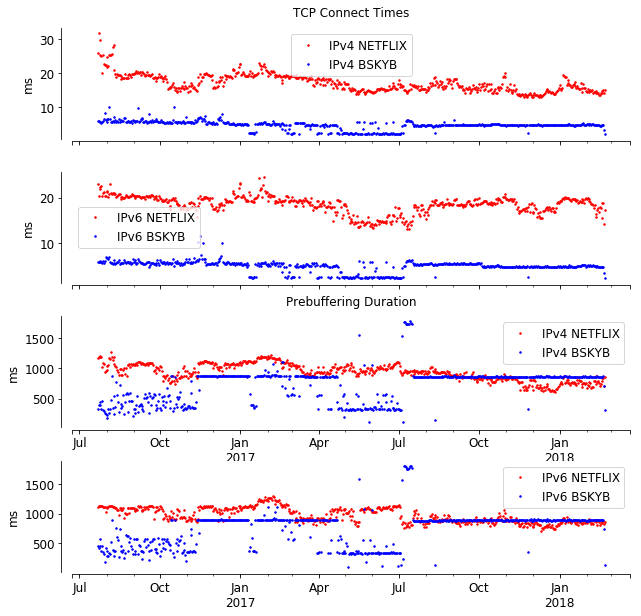
\includegraphics[keepaspectratio, height=8cm, width=15cm]{figures/cache/bskyb/netflix-tcp-pd-delay-timeseries-asn-5607-separate.png}
	\caption[SKY UK TCP Connect Times and Pre-Buffering Duration Timeseries Absolute]{Timeseries depicting the TCP connect times (\textit{connect\_time} field) and Prebuffering Duration (\textit{prebuffering\_duration} field) for SKY UK Limited against Netflix OCA servers. 
	We are applying a median aggregate here over the absolute values ans as can be seen, the TCP connect times is better for SKY UK Limited for both the address families. Prebuffering duration also shows the similar
	results until August 2017, after that the performance is comparable to Netflix OCA servers.}
	\label{fig: SKY UK TCP Connect Times and Pre-Buffering Duration Timeseries Absolute}
\end{figure}

We wanted to check if there is any benefits from the ISP content caches. Therfore, we identified the ISPs from all the holder names (refer \cref{table:asnname}) and tried to compare the performance
of an ISP cache with that of Netflix OCA servers. Here, the criteria we are using to identify a cache is when the AS number of the source IP address is same as the AS number of the destination IP address.
Therefore, the cache is identified when both the source and destination belongs to the same IP address. We started with the ISP named \textit{SKY UK Limited} \cite{skyuk}, as this is the
second ISP which contains the maximum number of distinct IPs (refer \cref{table:asnname}). We calcualted the Latency, Delay and Thoughput for this ISP with respect to Netflix (AS Number 2906).
After considering \textit{SKY UK Limited}, we did the similar analysis for two more cases, one of them is for the ISP \textit{British Telecommunications} \cite{btuk} which is also a major ISP in UK, the results for this ISP can be found in \hyperref[chapter:appendix]{Appendices}.
Also, \textit{British Telecommunications} has the third most number of distinct IPs in the dataset (refer \cref{table:asnname}). We then analysed the results for all ISPs content caches that were present in the dataset
against Netflix OCA servers.

\section{SKY UK Limted}

\subsection*{TCP Latency and Delay}

\begin{figure}[!ht]
	\centering
	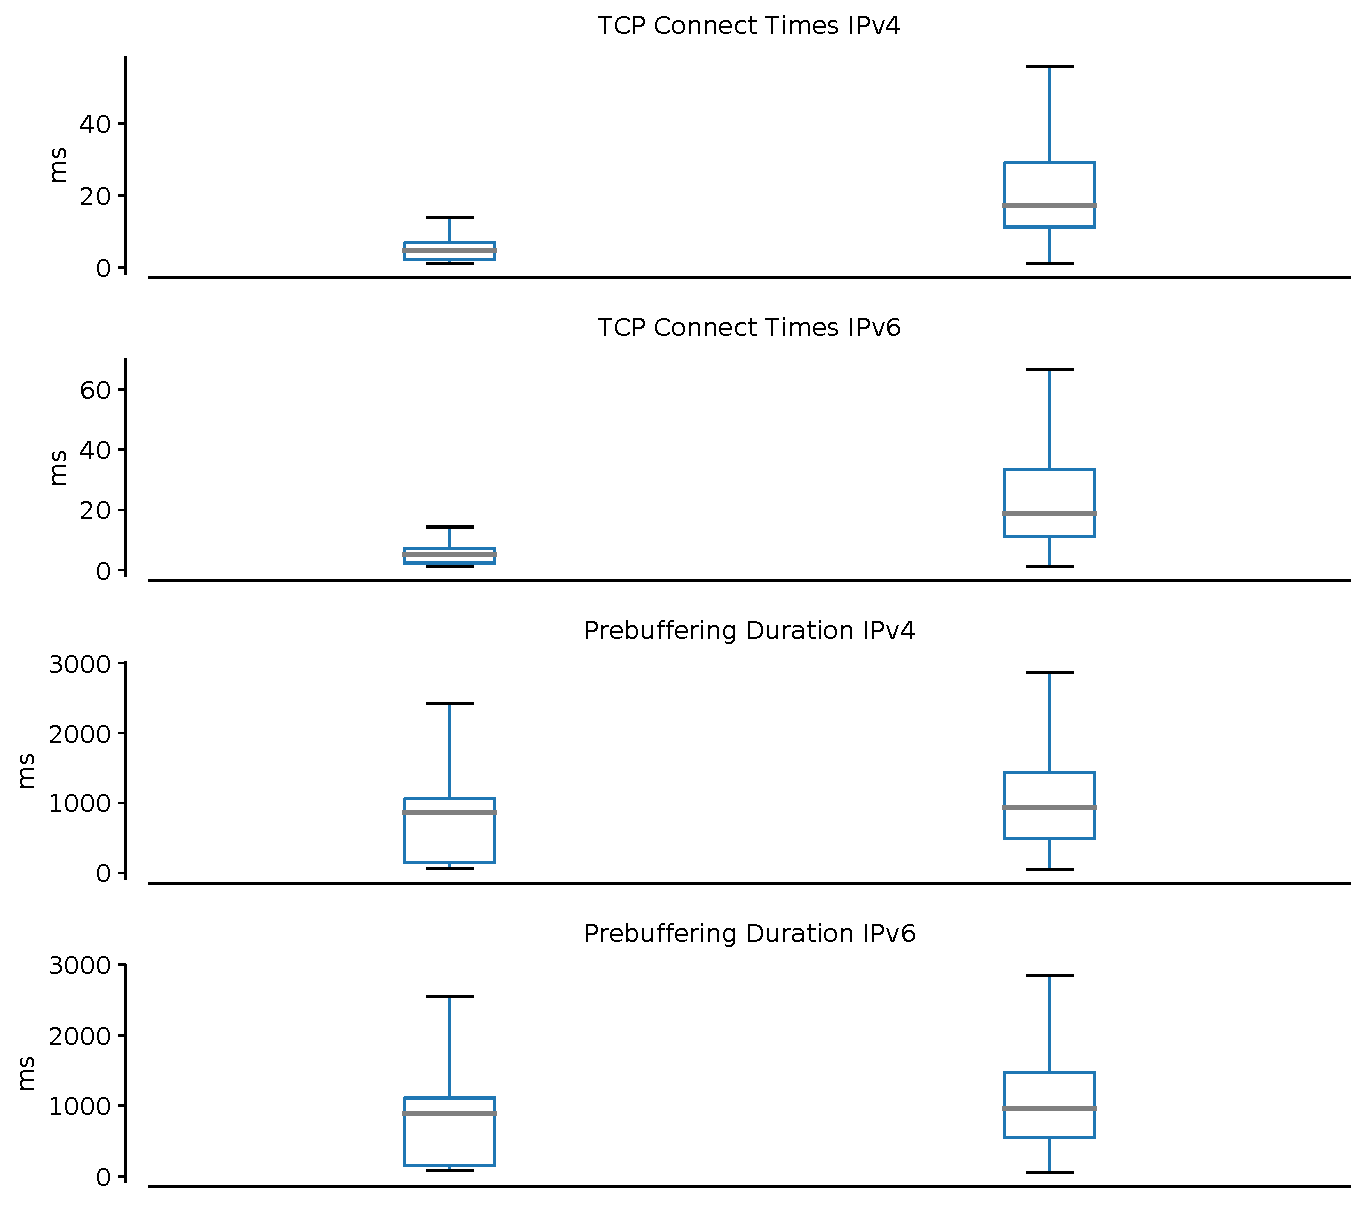
\includegraphics[keepaspectratio, height=8cm, width=15cm]{figures/cache/bskyb/netflix-tcp-prebuffering-delay-boxplot-bskyb-seprate.pdf}
	\caption[SKY UK TCP Connect Times and Pre-Buffering Duration Boxplot Absolute]{Boxplot depicting TCP connect times and Pre-Bufferring Duration for SKY UK Limited and Netflix. The median resemembles the Time series graph in \cref{fig:TCP Connect Times and Pre-Buffering Duration Timeseries Absolute}.}
	\label{fig: SKY UK TCP Connect Times and Pre-Buffering Duration Boxplot Absolute}
\end{figure}

\textit{SKY UK Limited} has the AS Number 5607, so for filtering out the rows which are using the criteria where both AS number of source IP address and AS number of destination IP address belongs to
the same As number which is 5607 here. Here, we are considering the \textit{connect\_time} and \textit{prebuffering\_duration} fields that are defined in \cref{table:netflix}. We first wanted to see how 
TCP connect times and prebuffering durations perform for both ISP caches and for Netflix (AS number 2906).
\cref{fig: SKY UK TCP Connect Times and Pre-Buffering Duration Timeseries Absolute} shows the timeseries for SKY UK Content caches and Netflix OCA servers over both the address families, 
and we have group by \textit{dtime} field and are considering the median aggregate here, so that a single vantage point doesn't bias the results.
As we can see, the TCP connect times is better for SKY UK Limited for both the address families, i.e. (0-10 ms), whereas for Netflix its around (0-30 ms). Prebuffering duration also shows the similar
results until August 2017, after that the performance is comparable to Netflix OCA servers. We have converted the connect time and pre-buffering duration to 'ms' to get a better understanding.
To get more clear view of the delays, we plot the boxplots for both SKY UK Limited and Netflix over Ipv4 and IPv6.  The median line in \cref{fig: SKY UK TCP Connect Times and Pre-Buffering Duration Boxplot Absolute}
graph resembles the timeseries in \cref{fig:Connect Time and Prebuffering Duration for IPv4 and IPv6 Timeseries}. Furthermore, the thrid quartile is pretty low for \textit{SKY UK Limited} content caches.
We further investigate the distribution of latency and delays for SKY UK and Netflix, here also, we filter the data along IPv4 and IPv6 and then take the CDF of the desired attributes. 
\cref{fig: SKY UK Connect Time and Prebuffering Duration CDF Absolute} shows the CDF of TCP connect times and prebuffering durations for SKY UK and Netflix. Around 80\% of the probes require TCP connect times of 19.5 ms
for SKY UK Limited over IPv4, whereas it'3 38.5 ms for the same number of probes for Netflix. Similarly, for IPv6, 80\% of the probes require 15.5 ms for SKY UK, whereas it is 40.75 ms for Netflix.
For pre-bufferind duration, SKY UK caches require around 1530 ms for 80\% of the probes over IPv4, and for Netflix the number is 1632 ms for same number of probes. For IPv6, SKY UK requires
1560 ms for 80\% of the probes and for Netflix the number is 1730 ms. It would be also good to compare the deltas i.e. the difference between the Latencies over IPv4 and IPv6 for SKY UK and Netflix.

\begin{figure}
	\centering
	\begin{minipage}{0.5\textwidth}
		\centering
		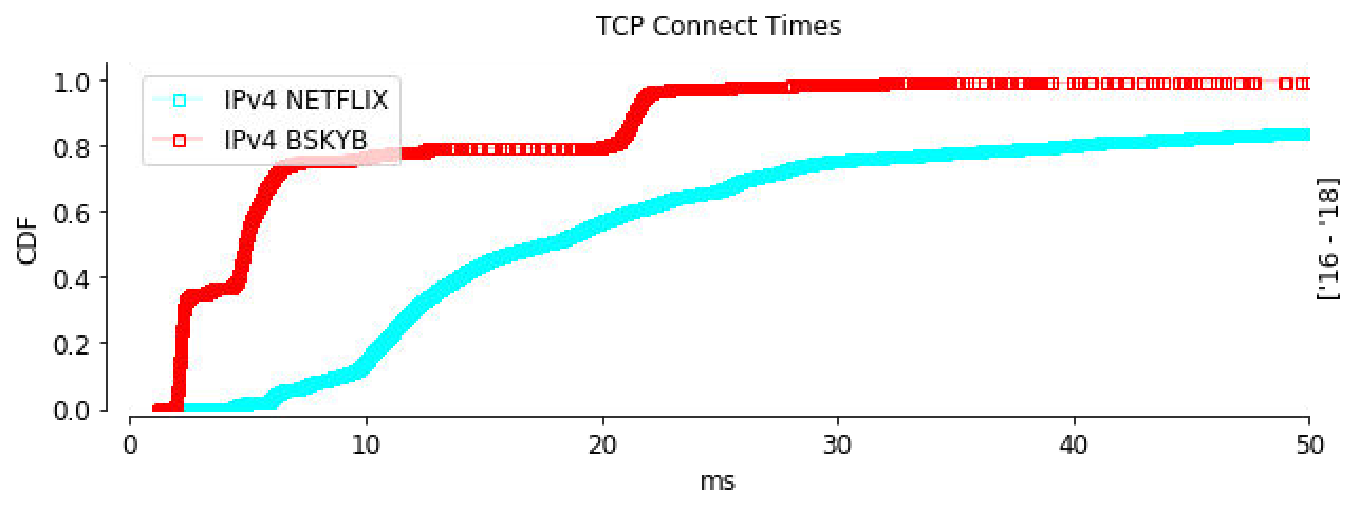
\includegraphics[keepaspectratio, height=5cm, width=8.5cm]{figures/cache/bskyb/netflix-syn-time-separate-bskyb-v4.pdf}
	\end{minipage}
	\begin{minipage}{0.5\textwidth}
		\centering
		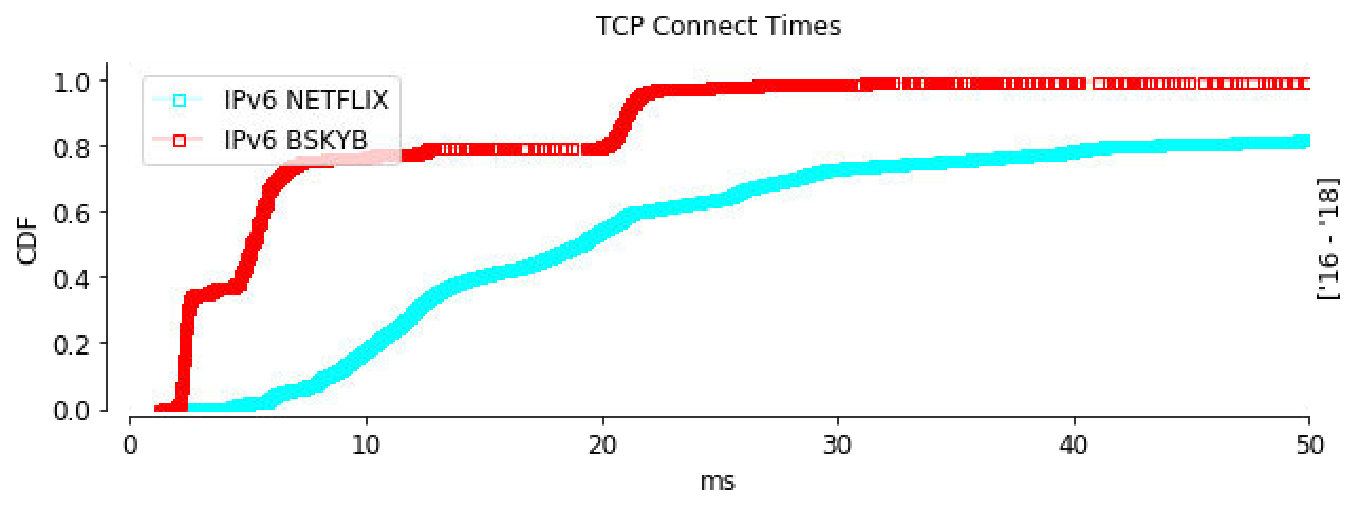
\includegraphics[keepaspectratio, height=5cm, width=8.5cm]{figures/cache/bskyb/netflix-syn-time-separate-bskyb-v6.pdf}
	\end{minipage}
	\begin{minipage}{0.5\textwidth}
		\centering
		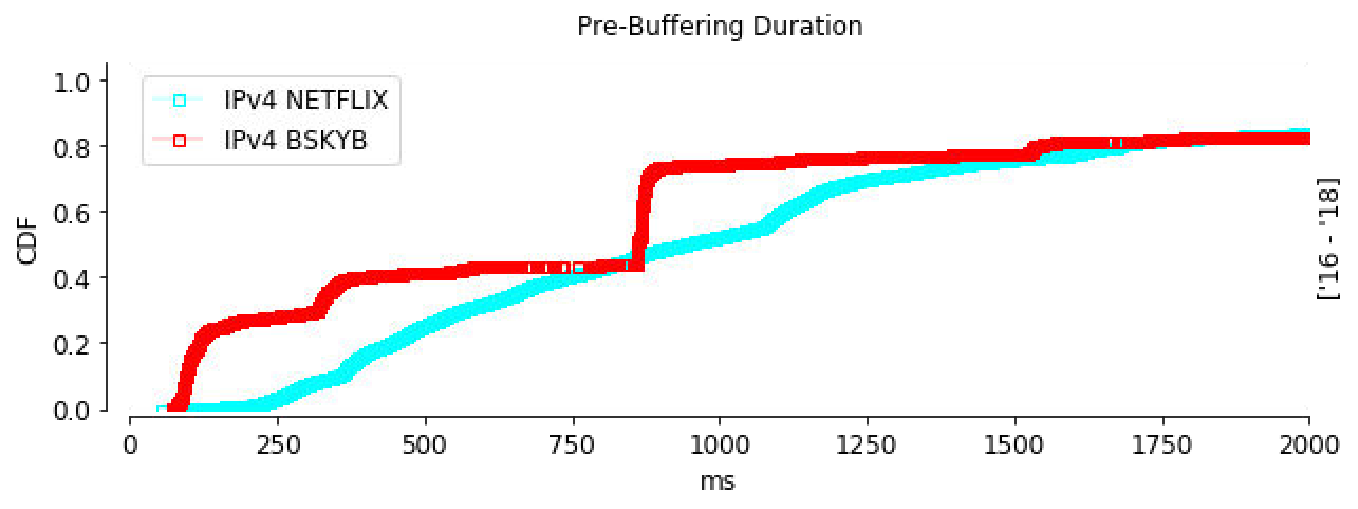
\includegraphics[keepaspectratio, height=5cm, width=8.5cm]{figures/cache/bskyb/netflix-prebuffering-duration-separate-bskyb-v4.pdf}
	\end{minipage}
	\begin{minipage}{0.5\textwidth}
		\centering
		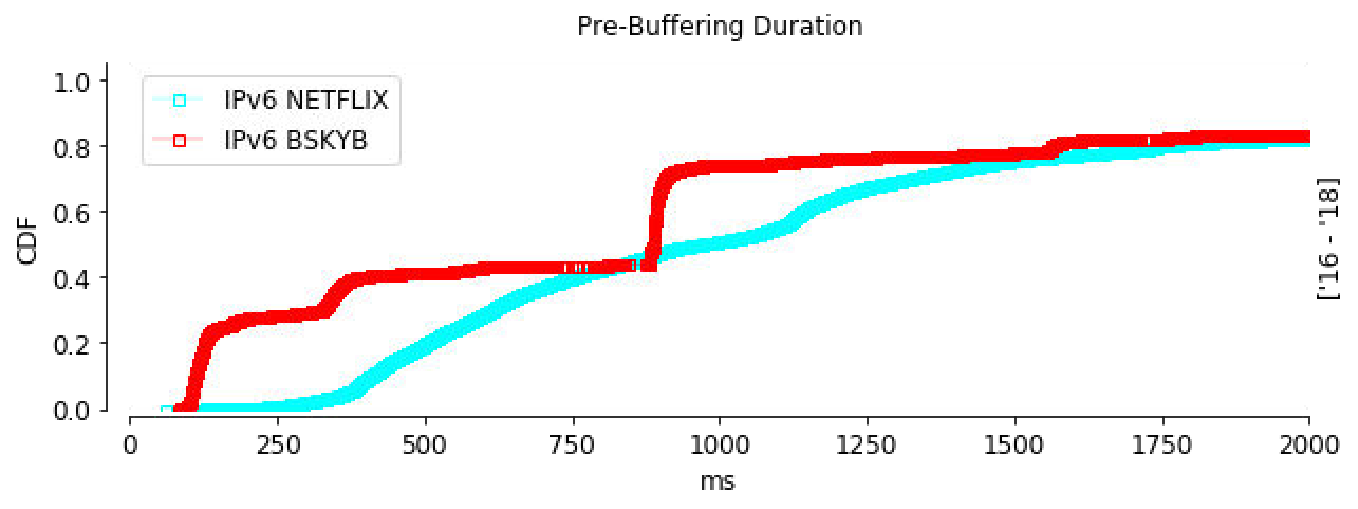
\includegraphics[keepaspectratio, height=5cm, width=8.5cm]{figures/cache/bskyb/netflix-prebuffering-duration-separate-bskyb-v6.pdf}
	\end{minipage}
	\caption[SKY UK Connect Time and Prebuffering Duration CDF Absolute]{CDF of TCP Connect times and Pre-Buffering duration for SKY UK Limited and Netflix over IPv4 and IPv6. As we can see, TCP COnnect times and Prebuffering duration for SKY UK Limited content caches is better than Netflix OCA servers.}
	\label{fig: SKY UK Connect Time and Prebuffering Duration CDF Absolute}
\end{figure}

\FloatBarrier

\begin{figure}[!ht]
	\centering
	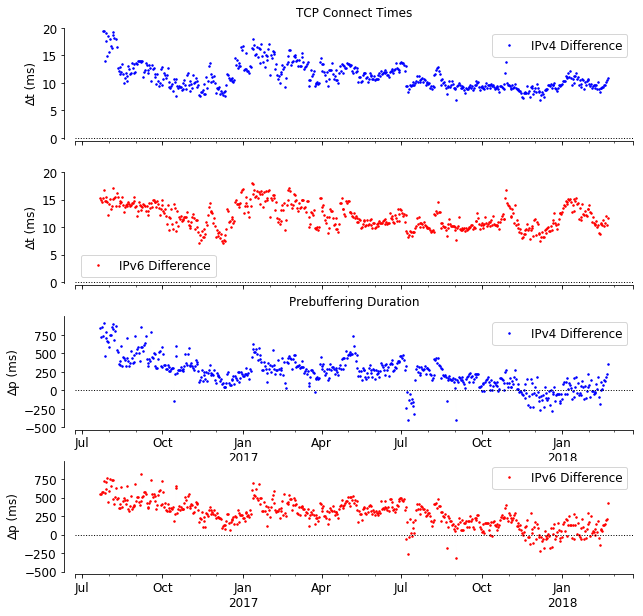
\includegraphics[keepaspectratio, height=8cm, width=15cm]{figures/cache/bskyb/netflix-tcp-pd-delay-timeseries-asn-5607.png}
	\caption[SKY UK TCP Connect Times and Pre-Buffering Duration Timeseries Deltas]{Time series of difference for TCP connect times and prebuffering durations over IPv4 and IPv6 between Netflix and SKY UK Limited. 
	Here, positive values indicate Netflix OCA server requires more connect time and pre-buffering duration as compared to SKY UK caches. Latency of around 10-15 ms and higher prebuffering durations (around 0-250 ms or more) are observed for Netflix over both IPv4 and IPv6.}
	\label{fig:SYK UK TCP Connect Times and Pre-Buffering Duration Timeseries Deltas}
\end{figure}

We will now compare the Deltas that is, difference between Netflix OCA server TCP connect times and SKY UK caches TCP connect times over IPv4 and IPv6. We will now define the
terminology that we are using here, let us say, TCP connect time over IPv4 for SKY UK is tp(y) and TCP connect time over IPv4 for Netflix is tp(x), then the \textit{delta} will be $\Delta$tp = tp(x) - tp(y). 
We did calculate these deltas for TCP connect times and Prebuffering duration for SKY UK and Netflix over IPv4 and IPv6.
Also, as already discussed in \cref{chapter:Datasets}, prebuffering duration takes into account DNS resolution times and TCP connect times. 
We will now analyse the deltas to check the benefits of ISP caches.

\begin{figure}[!ht]
	\centering
	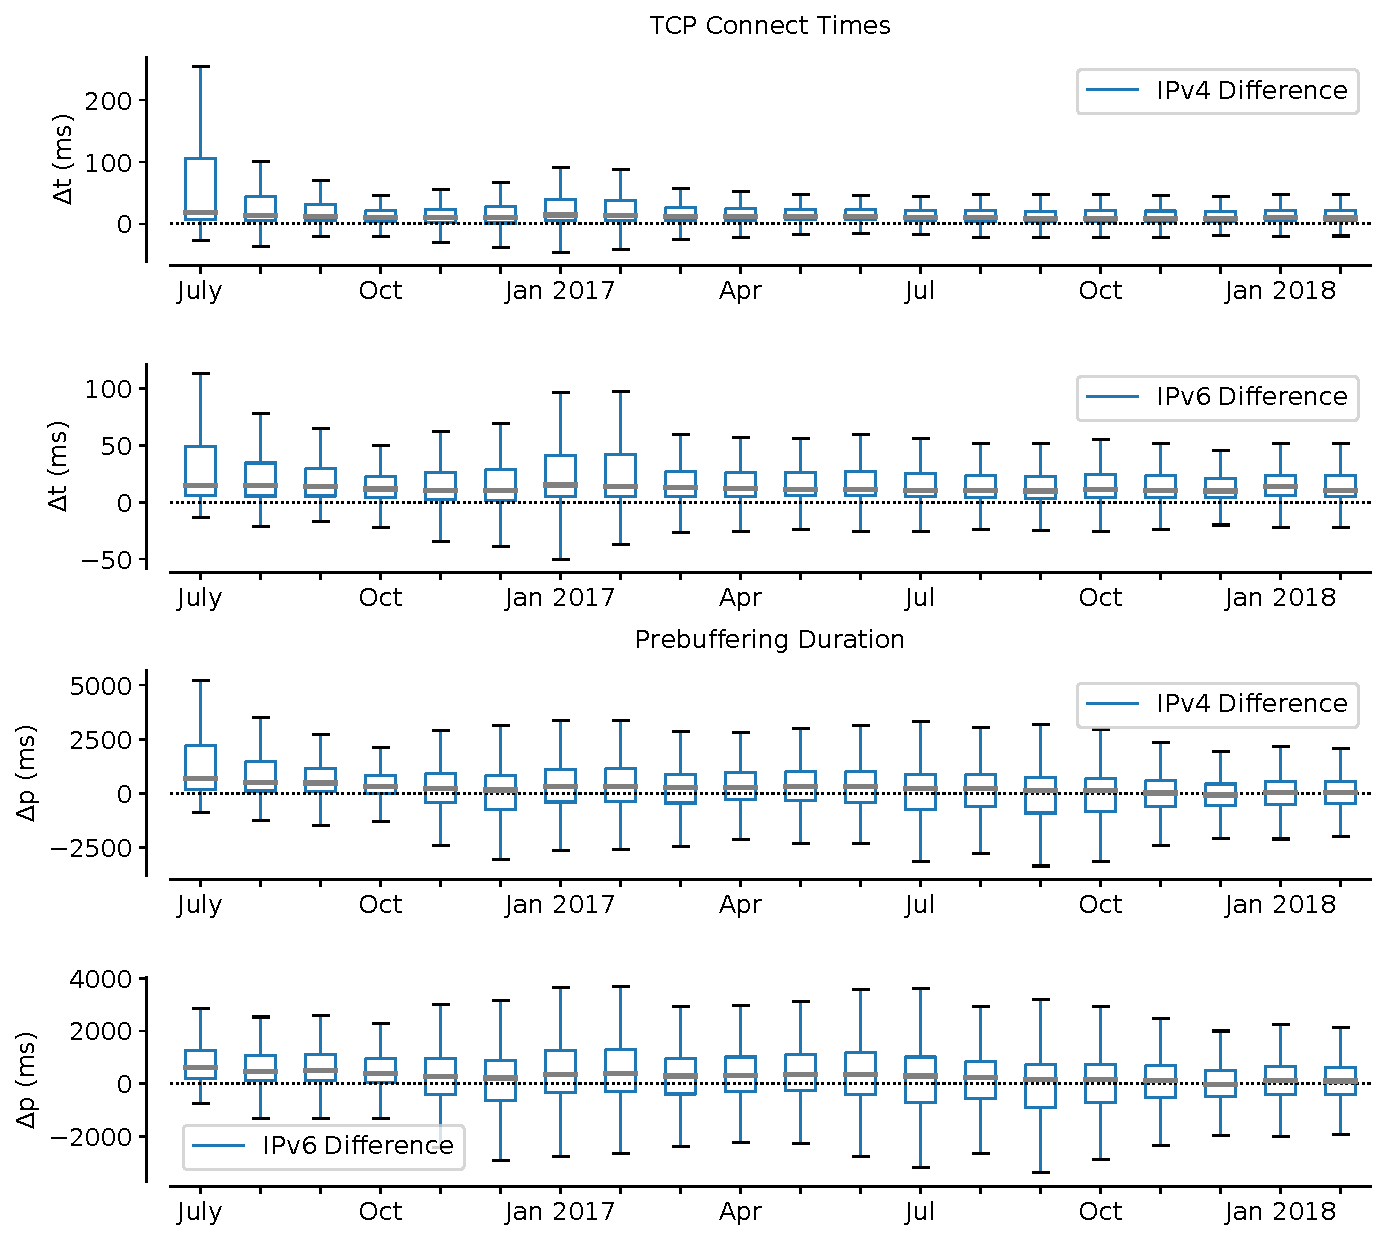
\includegraphics[keepaspectratio, height=8cm, width=15cm]{figures/cache/bskyb/netflix-tcp-pd-delay-boxplot-asn-5607.pdf}
	\caption[SKY UK TCP Connect Times and Pre-Buffering Duration Boxplot Deltas]{Boxplot of difference for TCP connect times and prebuffering durations over IPv4 and IPv6 between Netflix and SKY UK Limited.
	The median line here represents the time series graph in \cref{fig:SYK UK TCP Connect Times and Pre-Buffering Duration Timeseries Deltas}.}
	\label{fig:SKY UK TCP Connect Times and Pre-Buffering Duration Boxplot Deltas}
\end{figure}

To plot the deltas, we followed the same analysis \cite{bajpaimeasuring} did for the Youtueb dataset. To plot the timeseries for these deltas, we calculate the median aggregate on the
TCP connect times and the prebuffering duration across all probes on each day for the difference between Netflix and SKY UK limited.
\cref{fig:SYK UK TCP Connect Times and Pre-Buffering Duration Timeseries Deltas} shows the timeseries of median TCP connect times and prebuffering duration over IPv4 and IPv6 across all probes.
Here, positive values indicate Netflix OCA server requires more connect time and pre-buffering duration as compared to SKY UK caches. Latency of around 10-15 ms and higher prebuffering durations (around 0-250 ms or more) are observed for Netflix over both IPv4 and IPv6.
For boxplots in \cref{fig:SKY UK TCP Connect Times and Pre-Buffering Duration Boxplot Deltas}, we have rounded the time to the nearest month. Here, we can see that the median resembles the time series \cref{fig:SYK UK TCP Connect Times and Pre-Buffering Duration Timeseries Deltas}.
To get more vivid analysis, \cref{fig:SKY UK Connect Time and Prebuffering Duration CDF Deltas} shows us the distribution of difference in TCP connect times and prebuffering duration over the whole duration.
For calculating the CDF, we calcualted the deltas and then plotted their CDF. To compare the performance, 
we are measuring the TCP connect times to the Netflix OCA (Open Connect Appliances) server and to the SKY UK content caches, 
the distribution here shows that around 85\% of the connections are slower for Netflix OCA servers over IPv4 , and around 86\% of the connections are slower for Netflix over IPv6. 
For prebuffering duration which is the time to fetch 2 seconds of video at the specified bitrate from the content server, here Netflix OCA (Open Connect Appliances) server nad SKY Uk caches,
the distribution shows that 61\% of the connections are slower for Netflix over IPv4, and around 63\% of the connections are slower for Netflix over IPv6.

\begin{figure}
	\centering
	\begin{minipage}{0.5\textwidth}
		\centering
		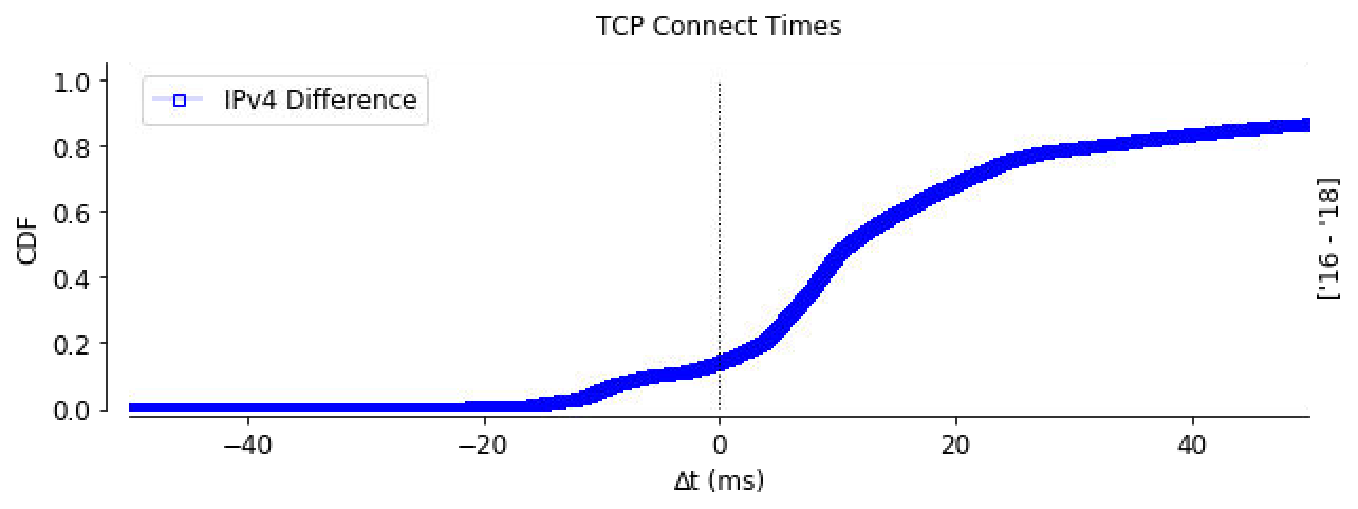
\includegraphics[keepaspectratio, height=5cm, width=8.5cm]{figures/cache/bskyb/netflix-syn-diff-5607-cdf-v4.pdf}
	\end{minipage}
	\begin{minipage}{0.5\textwidth}
		\centering
		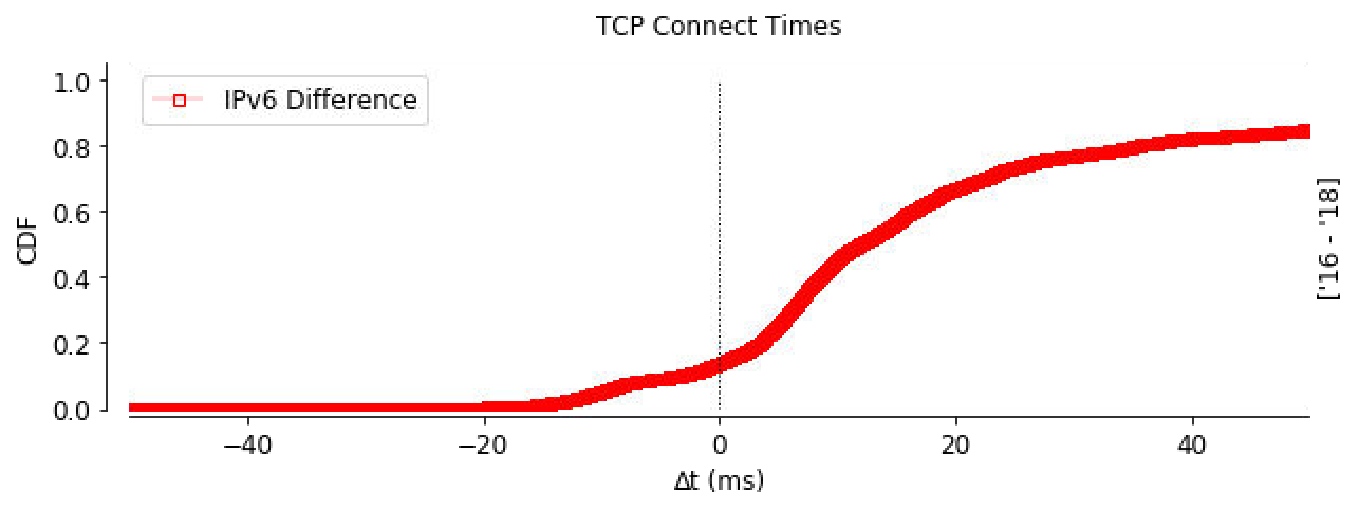
\includegraphics[keepaspectratio, height=5cm, width=8.5cm]{figures/cache/bskyb/netflix-syn-diff-5607-cdf-v6.pdf}
	\end{minipage}
	\begin{minipage}{0.5\textwidth}
		\centering
		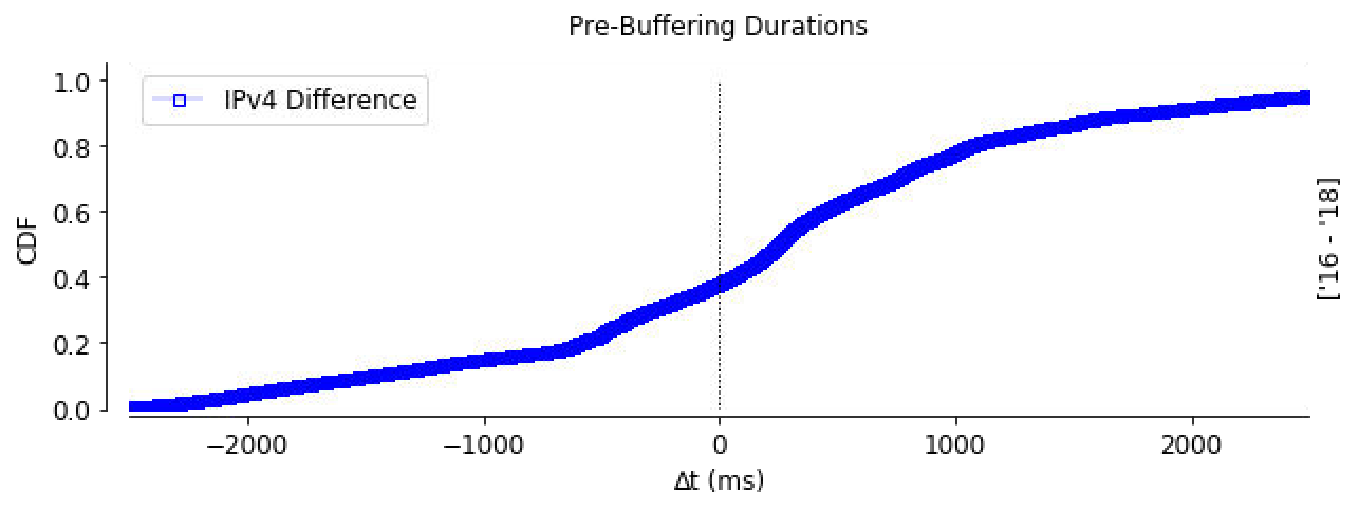
\includegraphics[keepaspectratio, height=5cm, width=8.5cm]{figures/cache/bskyb/netflix-pd-diff-5607-cdf-v4.pdf}
	\end{minipage}
	\begin{minipage}{0.5\textwidth}
		\centering
		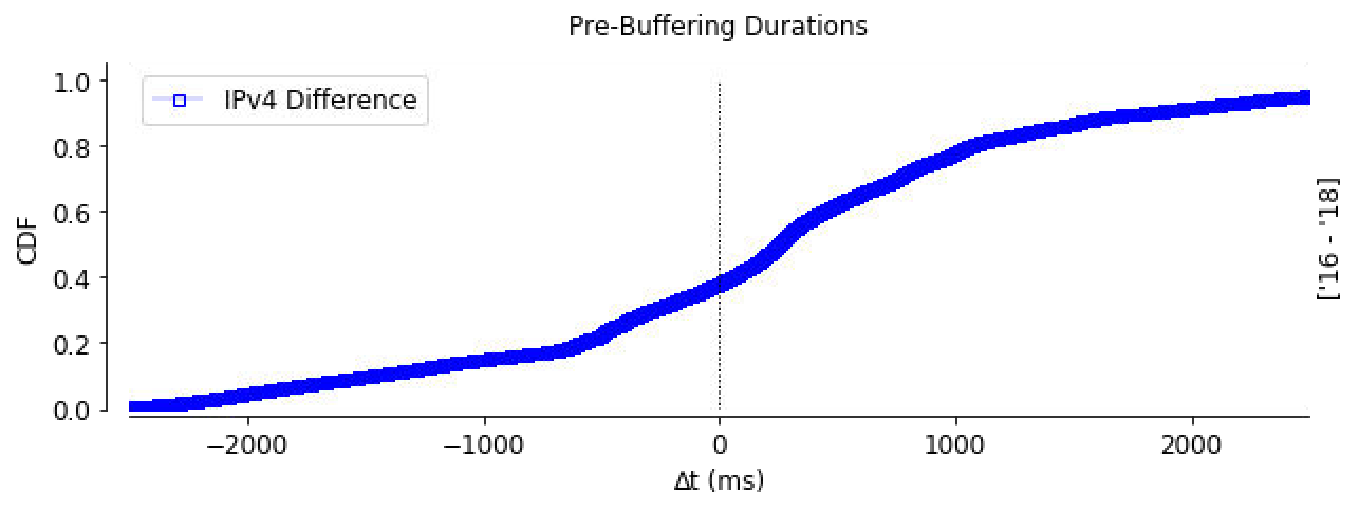
\includegraphics[keepaspectratio, height=5cm, width=8.5cm]{figures/cache/bskyb/netflix-pd-diff-5607-cdf-v4.pdf}
	\end{minipage}
	\caption[SKY UK Connect Time and Prebuffering Duration CDF Deltas]{CDF of difference of TCP connect times and Prebuffering Durations for Netflix and SKY UK over IPv4 and IPv6. The distribution here shows that around 85\% of the connections are slower for Netflix OCA servers over IPv4 , and around 86\% of the connections are slower for Netflix over IPv6. 
For prebuffering duration which is the time to fetch 2 seconds of video at the specified bitrate from the content server, here Netflix OCA (Open Connect Appliances) server nad SKY Uk caches,
the distribution shows that 61\% of the connections are slower for Netflix over IPv4, and around 63\% of the connections are slower for Netflix over IPv6.}
	\label{fig:SKY UK Connect Time and Prebuffering Duration CDF Deltas}
\end{figure}

\FloatBarrier

\subsection*{Throughput}

\begin{figure}[!ht]
	\centering
	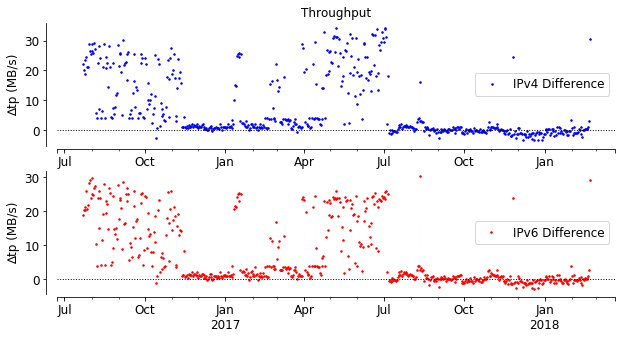
\includegraphics[keepaspectratio, height=5cm, width=15cm]{figures/cache/bskyb/netflix-throughput-timeseries-asn-5607.png}
	\caption[SKY UK Throughput Timeseries Absolute]{Time series of Throughput for individual address family's i.e. IPv4 and IPv6 for Netflix and SKY UK. We are considering 
	the \textit{bytes\_sec} field described in \cref{table:netflix}. As can be seen, the achieved throughput for SKY UK caches is somwehat comparable or more than Netflix OCA server, except after August 2017, where it is lower.}
	\label{fig:SKY UK Throughput Timeseries Absolute}
\end{figure}

\begin{figure}[!ht]
	\centering
	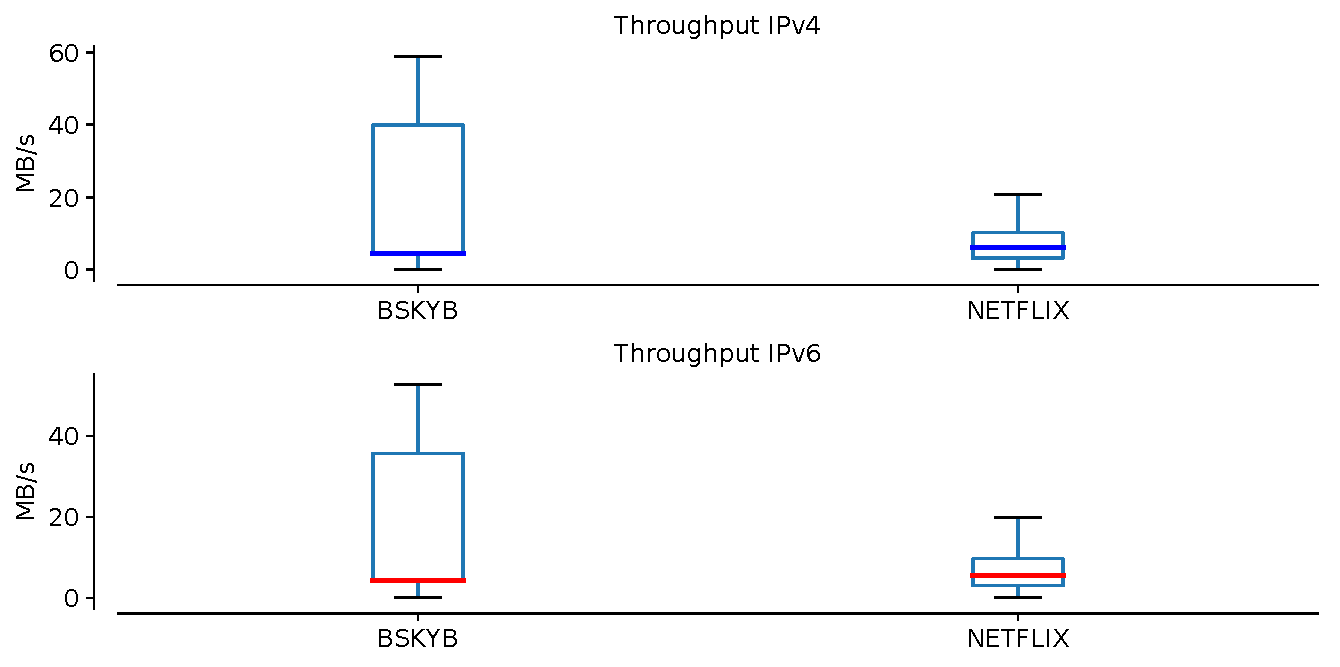
\includegraphics[keepaspectratio, height=5cm, width=15cm]{figures/cache/bskyb/netflix-throughput-boxplot-asn-5607-separate.pdf}
	\caption[SKY UK Throughput Boxplot Absolute]{Boxplot of Throughput for individual address family's i.e. IPv4 and Ipv6 for Netflix and SKY UK. The median line here shows that the achieved throguhput is
	comparable but the thrid quartile of SKY UK shows that the achieved throughput is higher for SKY UK over both address family's.}
	\label{fig:SKY UK Throughput Boxplot Absolute}
\end{figure}

After comparing the TCP connect times and Pre-Buffering duration for Netflix and SKY UK, we now know that clients take higher TCP connect times and prebuffering duration
for Netflix as compared to the SKY UK caches over both the address family's. We will now be comparing the achieved throughput over IPv4 and IPv6 for Netflix OCA server and SKY UK caches.
We will first look into the individual performance of IPv4 and IPv6 for Netflix and SKY UK and then will look into their deltas. \cref{fig:SKY UK Throughput Timeseries Absolute} gives the time series for
both the address families for SKY UK and Netflix,As can be seen, the achieved throughput for SKY UK caches is somwehat comparable or more than Netflix OCA server, except after August 2017, where it is lower.
We are considering the \textit{bytes\_sec} field from the Netflix \cref{table:netflix.}, and we are taking the median aggregate across
all probes on each day. Also, the throughput for IPv4 and IPv6 lies between 0-40 MB/s for SKY UK. To get more deeper insights
we also did the boxplot for IPv4 and IPv6 throughput for SKY UK and Netflix, and as can be seen in \cref{fig:SKY UK Throughput Boxplot Absolute} the monthly
throughput variation over IPv4 and IPv6. The median line here shows that the achieved throguhput is comparable but the thrid quartile of SKY UK shows that the achieved throughput is higher for SKY UK over both address family's. We have 
converted the \textit{bytes\_sec} field into MB/s to get a more realistic view. \cref{fig:SKY UK Throughput CDF Absolute} shows the CDF of
throughput over IPv4 and IPv6. We followed the same steps here, and plotted the CDF of \textit{bytes\_sec} field. The CDF here shows that around 80\% of the probes achieved a throughput of 42 MB/s for SKY UK over IPv4, whereas for Netflix this is only 11 MB/s
for similar number of probes. For IPv6, 80\% of the probes achieved the throughput of 36 MB/s, while for Netflix this was only 10 MB/s for similar number of probes. 
We will now look into the deltas to get better comparison between SKY UK and Netflix. 

\begin{figure}[!ht]
	\centering
	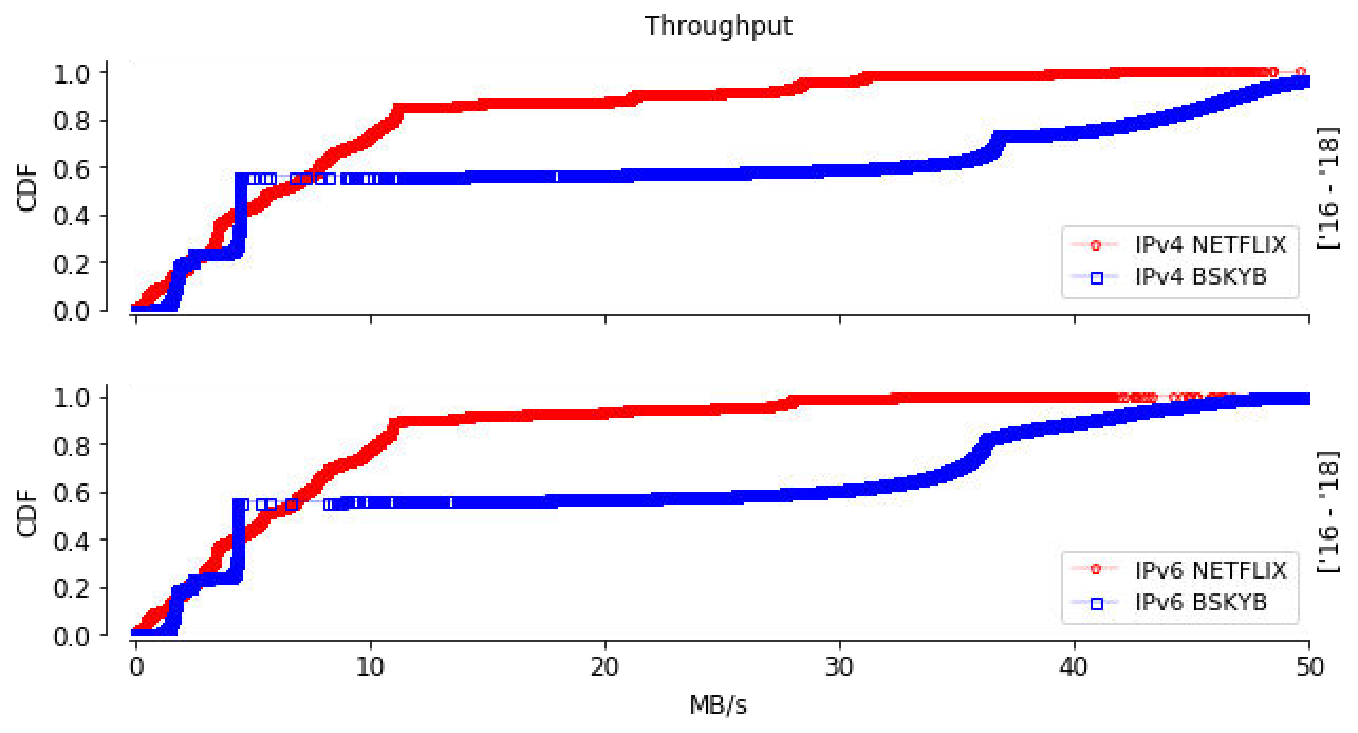
\includegraphics[keepaspectratio, height=5cm, width=15cm]{figures/cache/bskyb/netflix-throughput-difference-5607-separate.pdf}
	\caption[SKY UK Throughput CDF Absolute]{CDF of Throughput over IPv4 and IPv6 for SKY UK and Netflix. The CDF here shows that around 80\% of the probes achieved a throughput of 42 MB/s for SKY UK over IPv4, whereas for Netflix this is only 11 MB/s
for similar number of probes. For IPv6, 80\% of the probes achieved the throughput of 36 MB/s, while for Netflix this was only 10 MB/s for similar number of probes.}
	\label{fig:SKY UK Throughput CDF Absolute}
\end{figure}

\FloatBarrier

\begin{figure}[!ht]
	\centering
	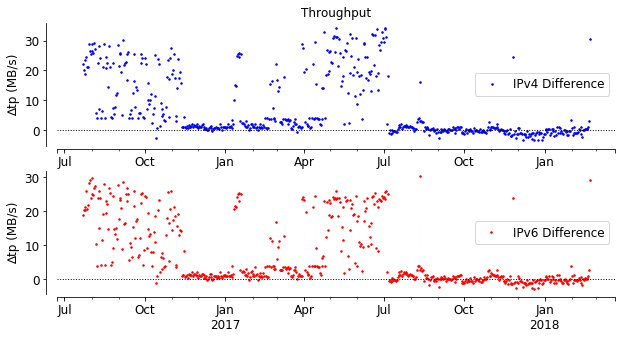
\includegraphics[keepaspectratio, height=5cm, width=15cm]{figures/cache/bskyb/netflix-throughput-timeseries-asn-5607.png}
	\caption[SKY UK Throughput Timeseries Deltas]{Time series of deltas of Throughput over IPv4 and IPv6 between SKY UK and Netflix. We can see that the difference is around 0 or more for the whole duration. 
The posiitive value indicates a higher throughput for SKY UK, also the difference lies between 0-30 MB/s.}
	\label{fig:SKY UK Throughput Timeseries Deltas}
\end{figure}

\begin{figure}[!ht]
	\centering
	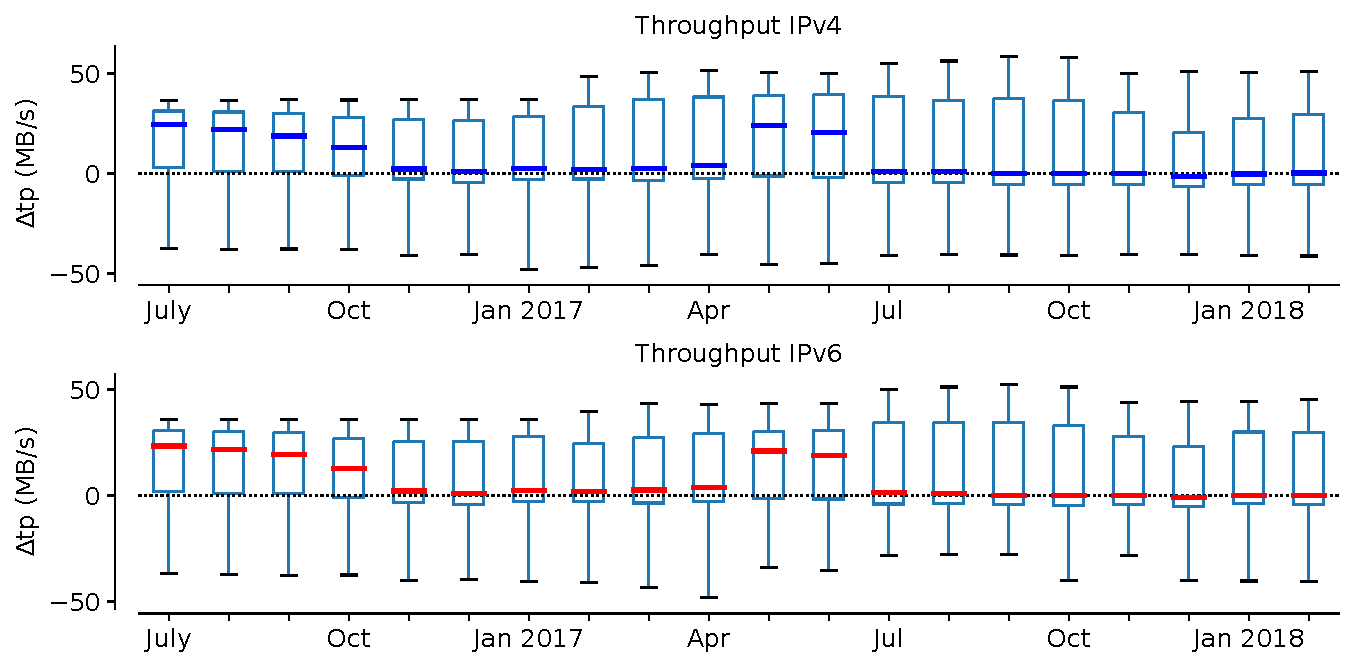
\includegraphics[keepaspectratio, height=5cm, width=15cm]{figures/cache/bskyb/netflix-throughput-boxplot-asn-5607.pdf}
	\caption[SKY UK Throughput Boxplot Deltas]{Boxplot of difference of throughput over IPv4 and IPv6 between SKY UK and Netflix. The median line shows similar curves as the time series \cref{fig:SKY UK Throughput Timeseries Deltas}, depicting higher throughput for SKy UK over both address families.}
	\label{fig:SKY UK Throughput Boxplot Deltas}
\end{figure}

Before starting with the deltas, we would live to define the terminologies we used to get the results. We are considering the \textit{bytes\_sec} field only and using the same terminilogy Bajpai et al. used in \cite{bajpaimeasuring}. We denote the throughput 
over IPv4 for SKY UK as \textit{tp(y}) and throughput over IPv4 for Netflix as \textit{tp(x)}, then the \textit{delta} will be $\Delta$tp = tp(y) - tp(x).
To plot the deltas, we first start with the time series, and \cref{fig:SKY UK Throughput Timeseries Deltas} shows us the time series of median aggregate of throughput across all probes over each day.
We can see that the difference is around 0 or more for the whole duration. The posiitive value indicates a higher throughput for SKY UK, also the difference lies between 0-30 MB/s.
\cref{fig:SKY UK Throughput Boxplot Deltas} shows the boxplot of difference of throughput over IPv4 and IPv6 between SKY UK and Netflix. The median line shows similar curves as the time series \cref{fig:SKY UK Throughput Timeseries Deltas}, depicting higher throughput for SKy UK over both address families.
To get a more clear picture about the performance, we plot the CDF of \textit{bytes\_sec} field. 
\cref{fig:SKY UK Throughput CDF Deltas} shows the CDF of difference of throughput over IPv4 and IPv6 for SKY UK and Netflix. 
Around 60\% of the times, SKY UK caches achieved higher throughput than Netflix over IPv4 and IPv6.

\begin{figure}[!ht]
	\centering
	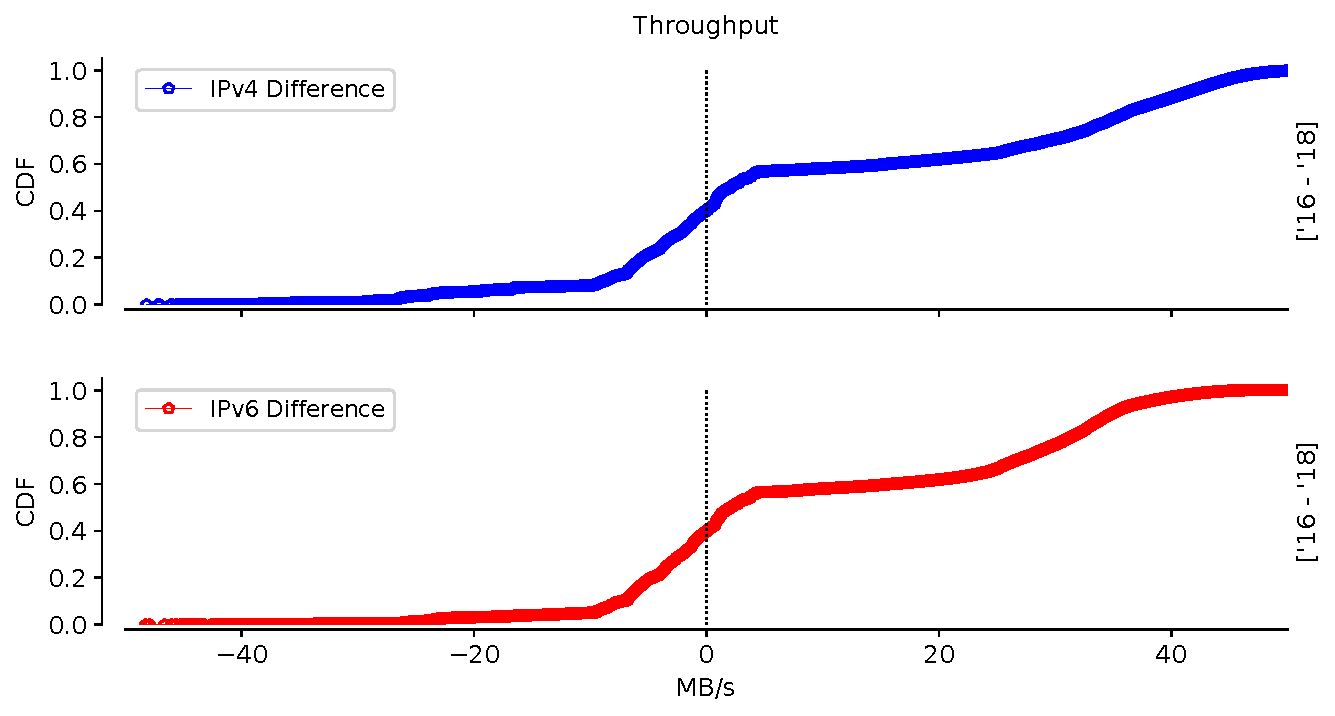
\includegraphics[keepaspectratio, height=5cm, width=15cm]{figures/cache/bskyb/netflix-throughput-difference-5607.pdf}
	\caption[SKY UK Throughput CDF Deltas]{CDF of difference of throughput over IPv4 and IPv6 for SKY UK and Netflix. 
Around 60\% of the times, SKY UK caches achieved higher throughput than Netflix over IPv4 and IPv6.}
	\label{fig:SKY UK Throughput CDF Deltas}
\end{figure}

\FloatBarrier

\section{All ISPs Together}

\begin{figure}[!ht]
	\centering
	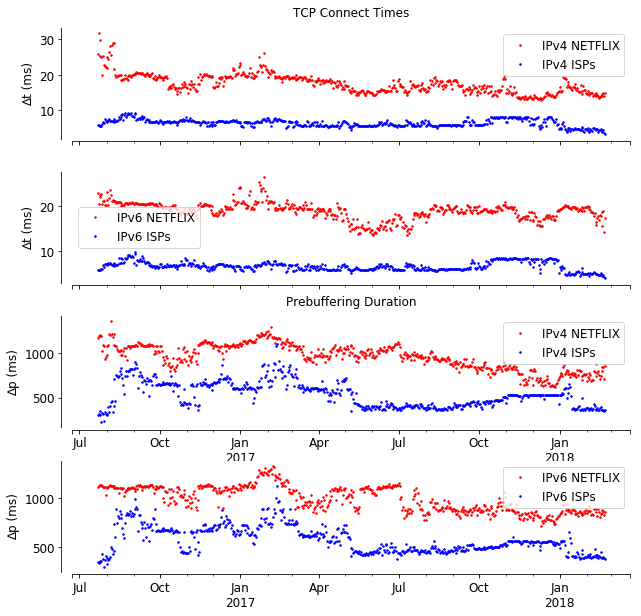
\includegraphics[keepaspectratio, height=8cm, width=15cm]{figures/cache/allisps/netflix-tcp-pd-delay-timeseries-all-isps-separate.png}
	\caption[All ISPs TCP Connect Times and Pre-Buffering Duration Timeseries Absolute]{Timeseries depicting the TCP connect times (\textit{connect\_time} field) and Prebuffering Duration (\textit{prebuffering\_duration} field) for all ISPs caches against Netflix OCA servers. 
	We are applying a median aggregate here over the absolute values and as can be seen, the TCP connect times is better for ISPs for both the address families. Prebuffering duration also shows the similar
	results i.e. ISP caches performs better here as well.}
	\label{fig:All ISPs TCP Connect Times and Pre-Buffering Duration Timeseries Absolute}
\end{figure}


SKY UK was one of the ISP we considered till now, we wanted to see how Netflix compares against all the ISPs content caches. So, here we are grouping all the ISPs mentioned in  \cref{table:asnname}.
We included all the ISPs belonging to this table. We know will compare All ISPs content caches against Netflix for the TCP connect times, Prebuffering duration and achieved throughput.

\subsection*{TCP Latency and Delay}

\begin{figure}[!ht]
	\centering
	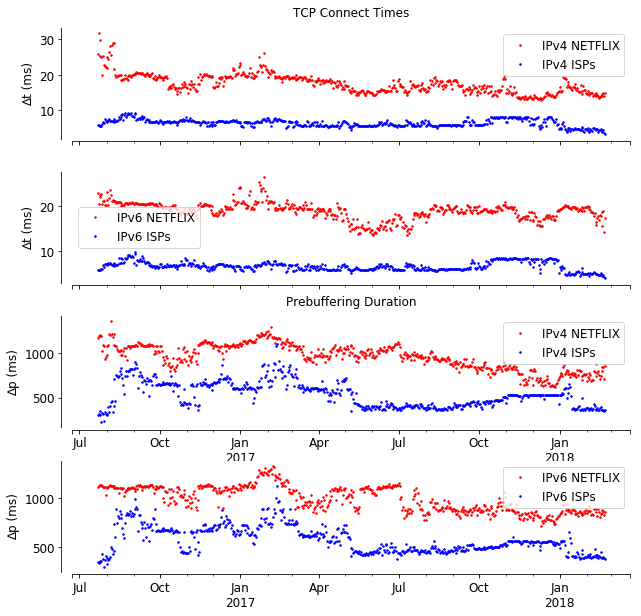
\includegraphics[keepaspectratio, height=8cm, width=15cm]{figures/cache/allisps/netflix-tcp-pd-delay-timeseries-all-isps-separate.png}
	\caption[All ISPs TCP Connect Times and Pre-Buffering Duration Timeseries Absolute]{Timeseries depicting the TCP connect times (\textit{connect\_time} field) and Prebuffering Duration (\textit{prebuffering\_duration} field) for all ISPs caches against Netflix OCA servers. 
	We are applying a median aggregate here over the absolute values and as can be seen, the TCP connect times is better for ISPs for both the address families. Prebuffering duration also shows the similar
	results i.e. ISP caches performs better here as well.}
	\label{fig:All ISPs TCP Connect Times and Pre-Buffering Duration Timeseries Absolute}
\end{figure}

\begin{figure}[!ht]
	\centering
	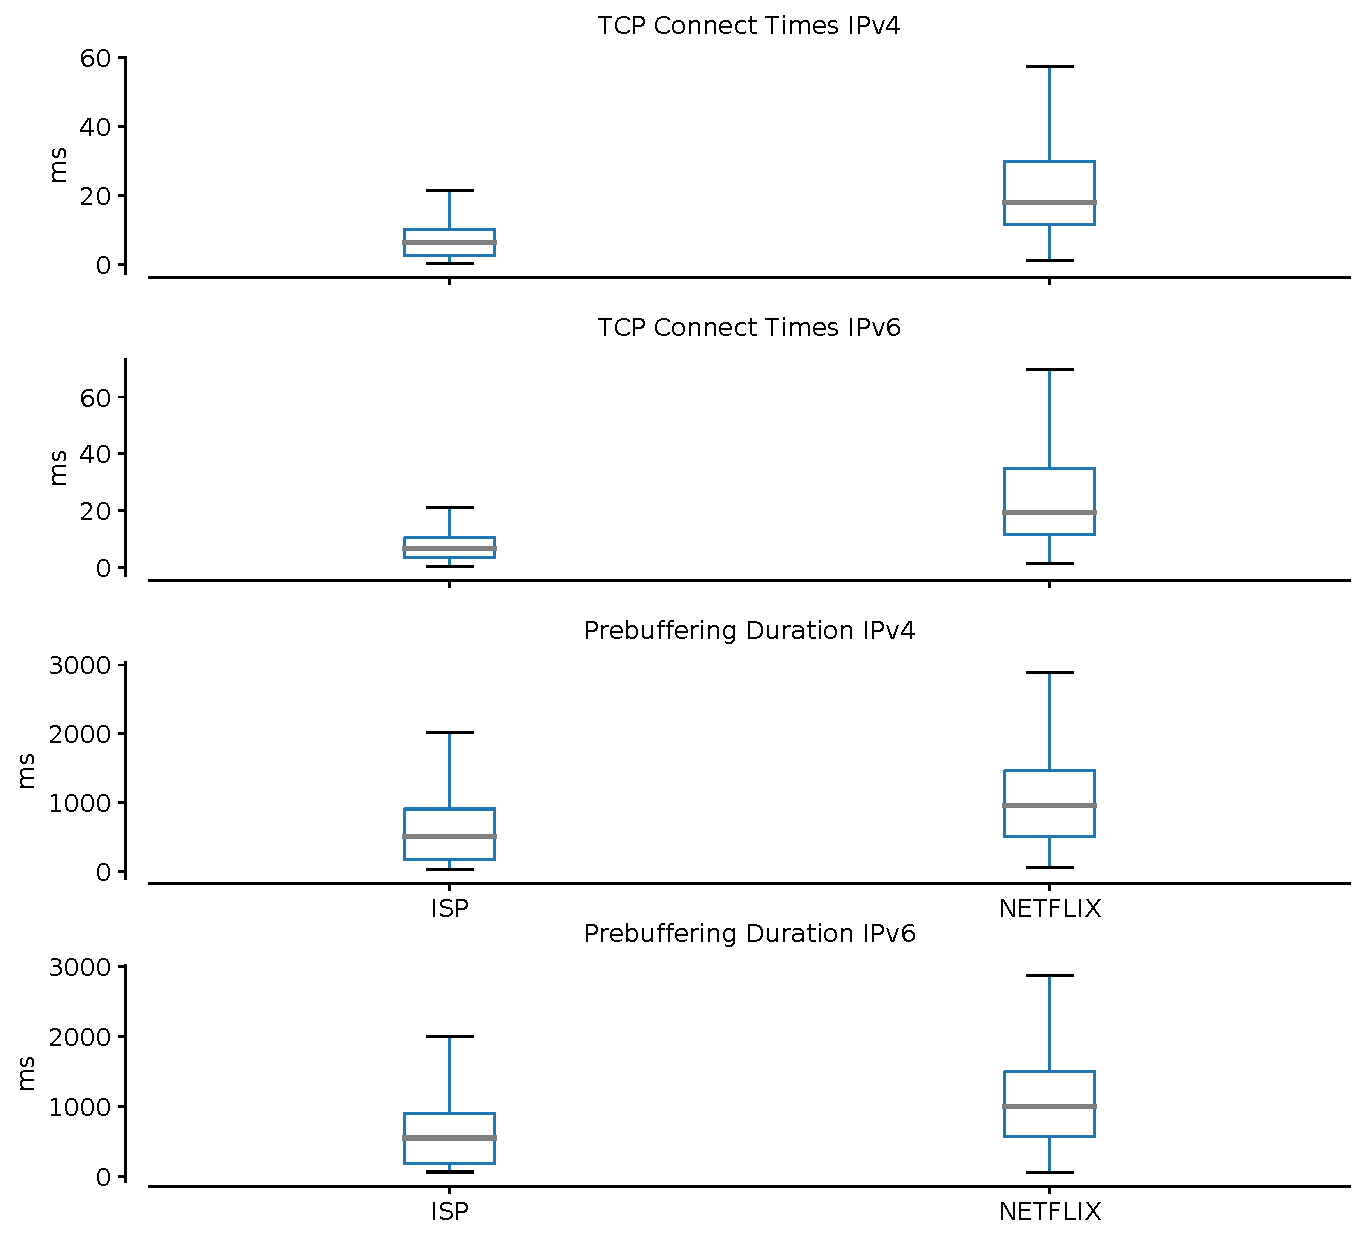
\includegraphics[keepaspectratio, height=8cm, width=15cm]{figures/cache/allisps/netflix-tcp-prebuffering-delay-boxplot-isps-seprate.pdf}
	\caption[ALL ISPs TCP Connect Times and Pre-Buffering Duration Boxplot Absolute]{Boxplot depicting TCP connect times and Pre-Bufferring Duration for ISPs and Netflix. The median resemembles the Time series graph in \cref{fig:All ISPs TCP Connect Times and Pre-Buffering Duration Timeseries Absolute}.}
	\label{fig:ALL ISPs TCP Connect Times and Pre-Buffering Duration Boxplot Absolute}
\end{figure}

Here, all ISPs are grouped together and we are using the criteria where both AS number of source IP address and AS number of destination IP address belongs to
the same AS number. We are considering the \textit{connect\_time} and \textit{prebuffering\_duration} fields that are defined in \cref{table:netflix}. We first wanted to see how 
TCP connect times and prebuffering durations perform for both ISP caches and for Netflix (AS number 2906).
\cref{fig:All ISPs TCP Connect Times and Pre-Buffering Duration Timeseries Absolute} shows the timeseries for all ISPs content caches and Netflix OCA servers over both the address families, 
and we have group by \textit{dtime} field and are considering the median aggregate here, so that a single vantage point doesn't bias the results.
As we can see, the TCP connect times is better for ISPs for both the address families, i.e. (0-10 ms), whereas for Netflix its around (0-30 ms). Prebuffering duration also shows the similar
results i.e. ISP caches performs better here as well. We have converted the connect time and pre-buffering duration to 'ms' to get a better understanding.
To get more clear view of the delays, we plot the boxplots for both ISPs and Netflix over IPv4 and IPv6.  The median line in \cref{fig:ALL ISPs TCP Connect Times and Pre-Buffering Duration Boxplot Absolute}
graph resembles the timeseries in \cref{fig:All ISPs TCP Connect Times and Pre-Buffering Duration Timeseries Absolute}. Furthermore, the thrid quartile is pretty low for \textit{ISPs} content caches.
We further investigate the distribution of latency and delays for ISPs and Netflix, here also, we filter the data along IPv4 and IPv6 and then take the CDF of the desired attributes. 
\cref{fig:ALL ISPs Connect Time and Prebuffering Duration CDF Absolute} shows the CDF of TCP connect times and prebuffering durations for the ISPs and Netflix. Around 80\% of the probes require TCP connect times of 13 ms
for ISPs over IPv4, whereas it's 38 ms for the same number of probes for Netflix. Similarly, for IPv6, 80\% of the probes require 14 ms for ISPs, whereas it is 41 ms for Netflix.
For pre-buffering duration, ISPs caches require around 1243 ms for 80\% of the probes over IPv4, and for Netflix the number is 1671 ms for same number of probes. For IPv6, ISPs caches requires
1275 ms for 80\% of the probes and for Netflix the number is 1738 ms. It would be also good to compare the deltas i.e. the difference between the Latencies over IPv4 and IPv6 for ISPs and Netflix.

\begin{figure}
	\centering
	\begin{minipage}{0.5\textwidth}
		\centering
		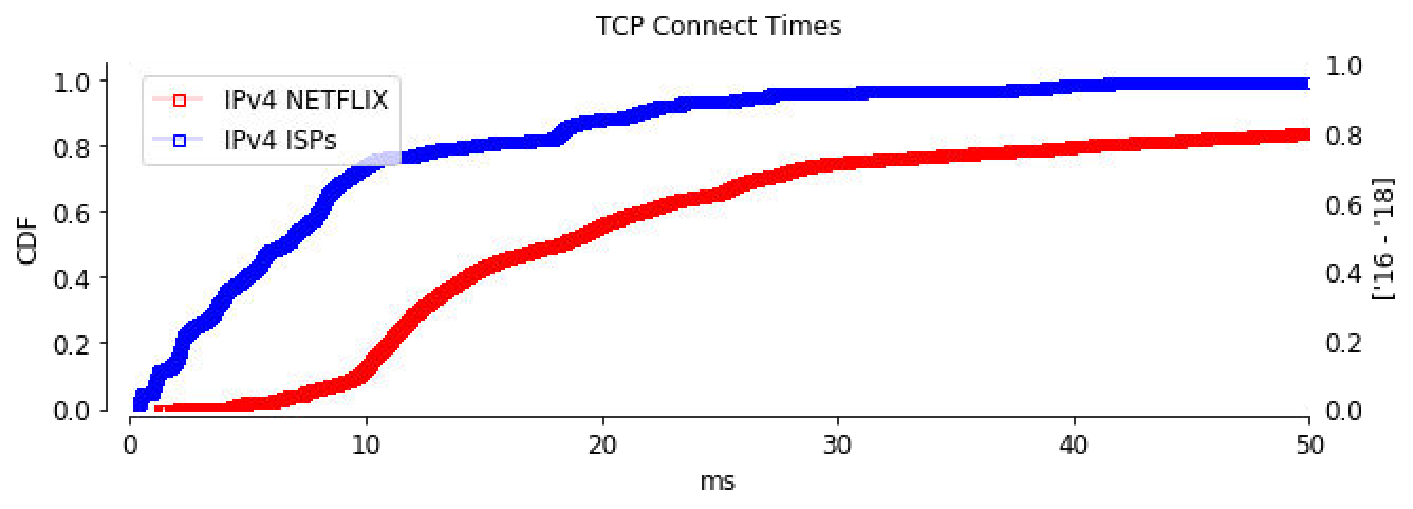
\includegraphics[keepaspectratio, height=5cm, width=8.5cm]{figures/cache/allisps/netflix-syn-time-separate-all-isps-v4.pdf}
	\end{minipage}
	\begin{minipage}{0.5\textwidth}
		\centering
		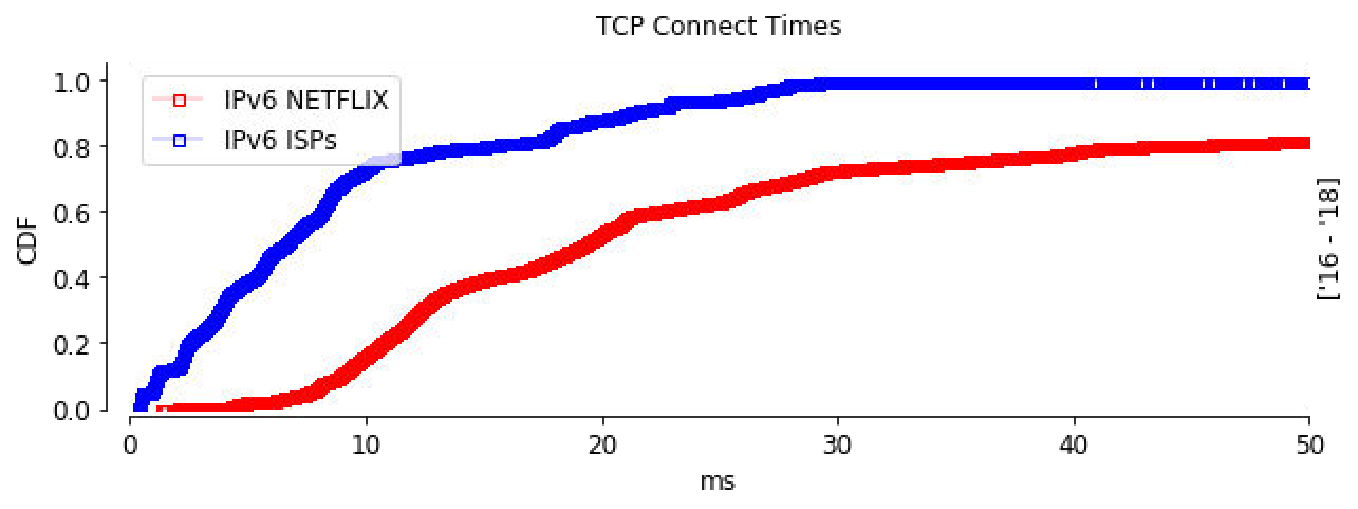
\includegraphics[keepaspectratio, height=5cm, width=8.5cm]{figures/cache/allisps/netflix-syn-time-separate-all-isps-v6.pdf}
	\end{minipage}
	\begin{minipage}{0.5\textwidth}
		\centering
		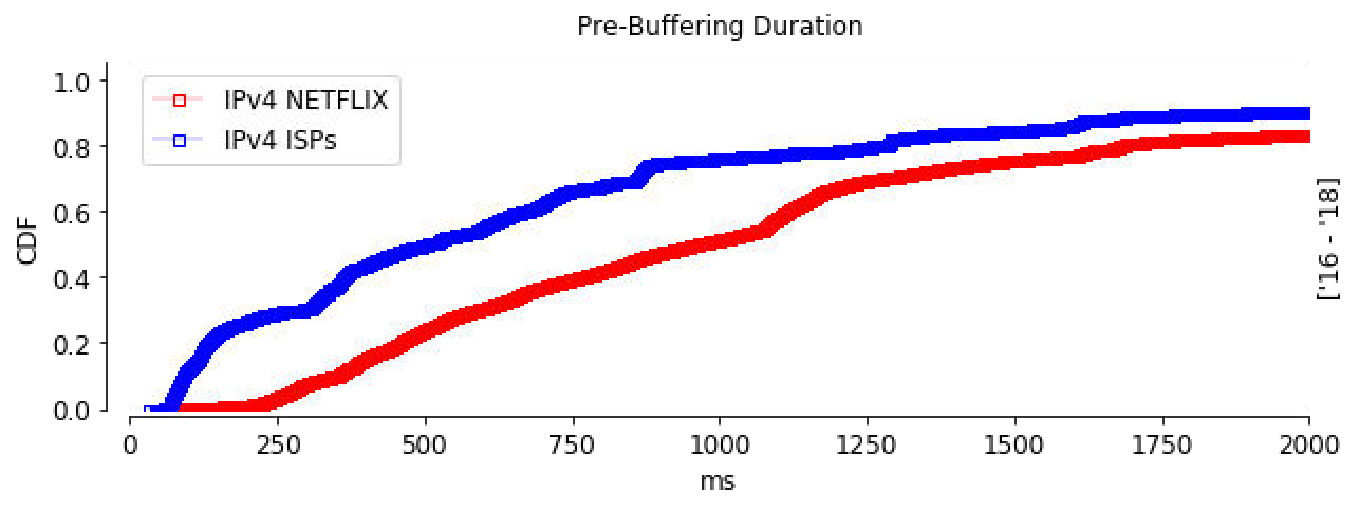
\includegraphics[keepaspectratio, height=5cm, width=8.5cm]{figures/cache/allisps/netflix-prebuffering-duration-separate-all-isps-v4.pdf}
	\end{minipage}
	\begin{minipage}{0.5\textwidth}
		\centering
		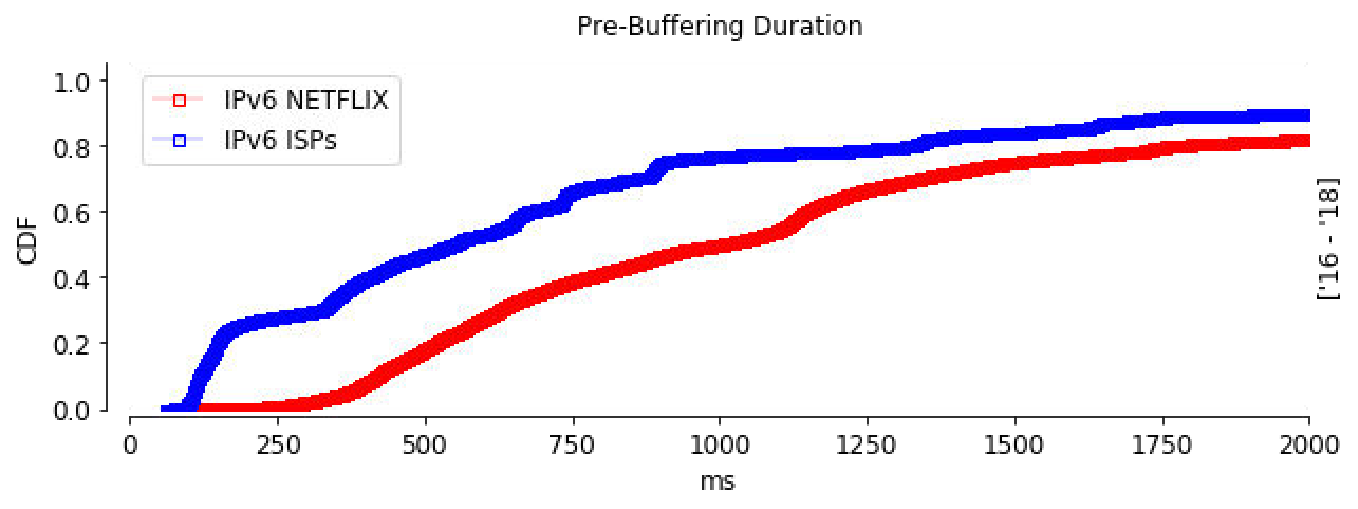
\includegraphics[keepaspectratio, height=5cm, width=8.5cm]{figures/cache/allisps/netflix-prebuffering-duration-separate-all-isps-v6.pdf}
	\end{minipage}
	\caption[All ISPs Connect Time and Prebuffering Duration CDF Absolute]{CDF of TCP Connect times and Pre-Buffering duration for all ISPs and Netflix over IPv4 and IPv6. As we can see, TCP Connect times and Prebuffering duration for ISPs content caches is better than Netflix OCA servers.}
	\label{fig:ALL ISPs Connect Time and Prebuffering Duration CDF Absolute}
\end{figure}

\FloatBarrier

\begin{figure}[!ht]
	\centering
	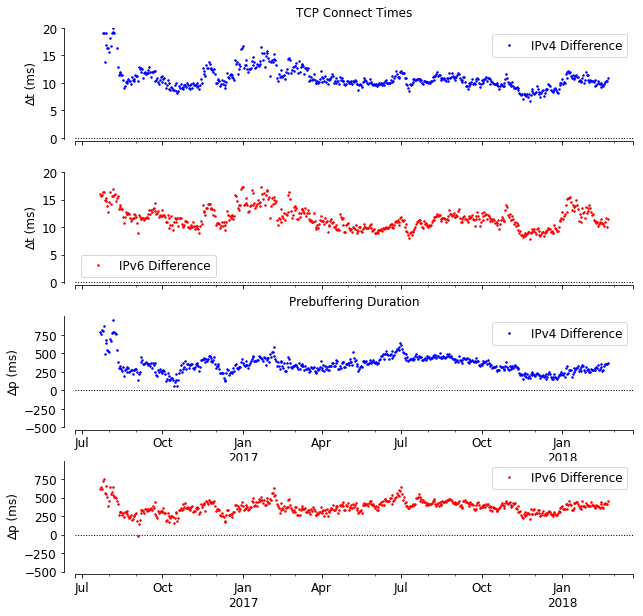
\includegraphics[keepaspectratio, height=8cm, width=15cm]{figures/cache/allisps/netflix-tcp-pd-delay-timeseries-all-isp.png}
	\caption[All ISPs TCP Connect Times and Pre-Buffering Duration Timeseries Deltas]{Time series of difference for TCP connect times and prebuffering durations over IPv4 and IPv6 between Netflix and ISPs. 
	Here, positive values indicate Netflix OCA server requires more connect time and pre-buffering duration as compared to ISPs caches. 
	Latency of around 10-20 ms and higher prebuffering durations (around 0-750 ms or more) are observed for Netflix over both IPv4 and IPv6.}
	\label{fig:All ISPs TCP Connect Times and Pre-Buffering Duration Timeseries Deltas}
\end{figure}

We will now compare the Deltas that is, difference between Netflix OCA server TCP connect times and ISPs caches TCP connect times over IPv4 and IPv6. We will now define the
terminology that we are using here, let us say, TCP connect time over IPv4 for ISPs is tp(y) and TCP connect time over IPv4 for Netflix is tp(x), then the \textit{delta} will be $\Delta$tp = tp(x) - tp(y). 
We did calculate these deltas for TCP connect times and Prebuffering duration for ISPs and Netflix over IPv4 and IPv6.
Also, as already discussed in \cref{chapter:Datasets}, prebuffering duration takes into account DNS resolution times and TCP connect times. 
We will now analyse the deltas to check the benefits of ISP caches.

\begin{figure}[!ht]
	\centering
	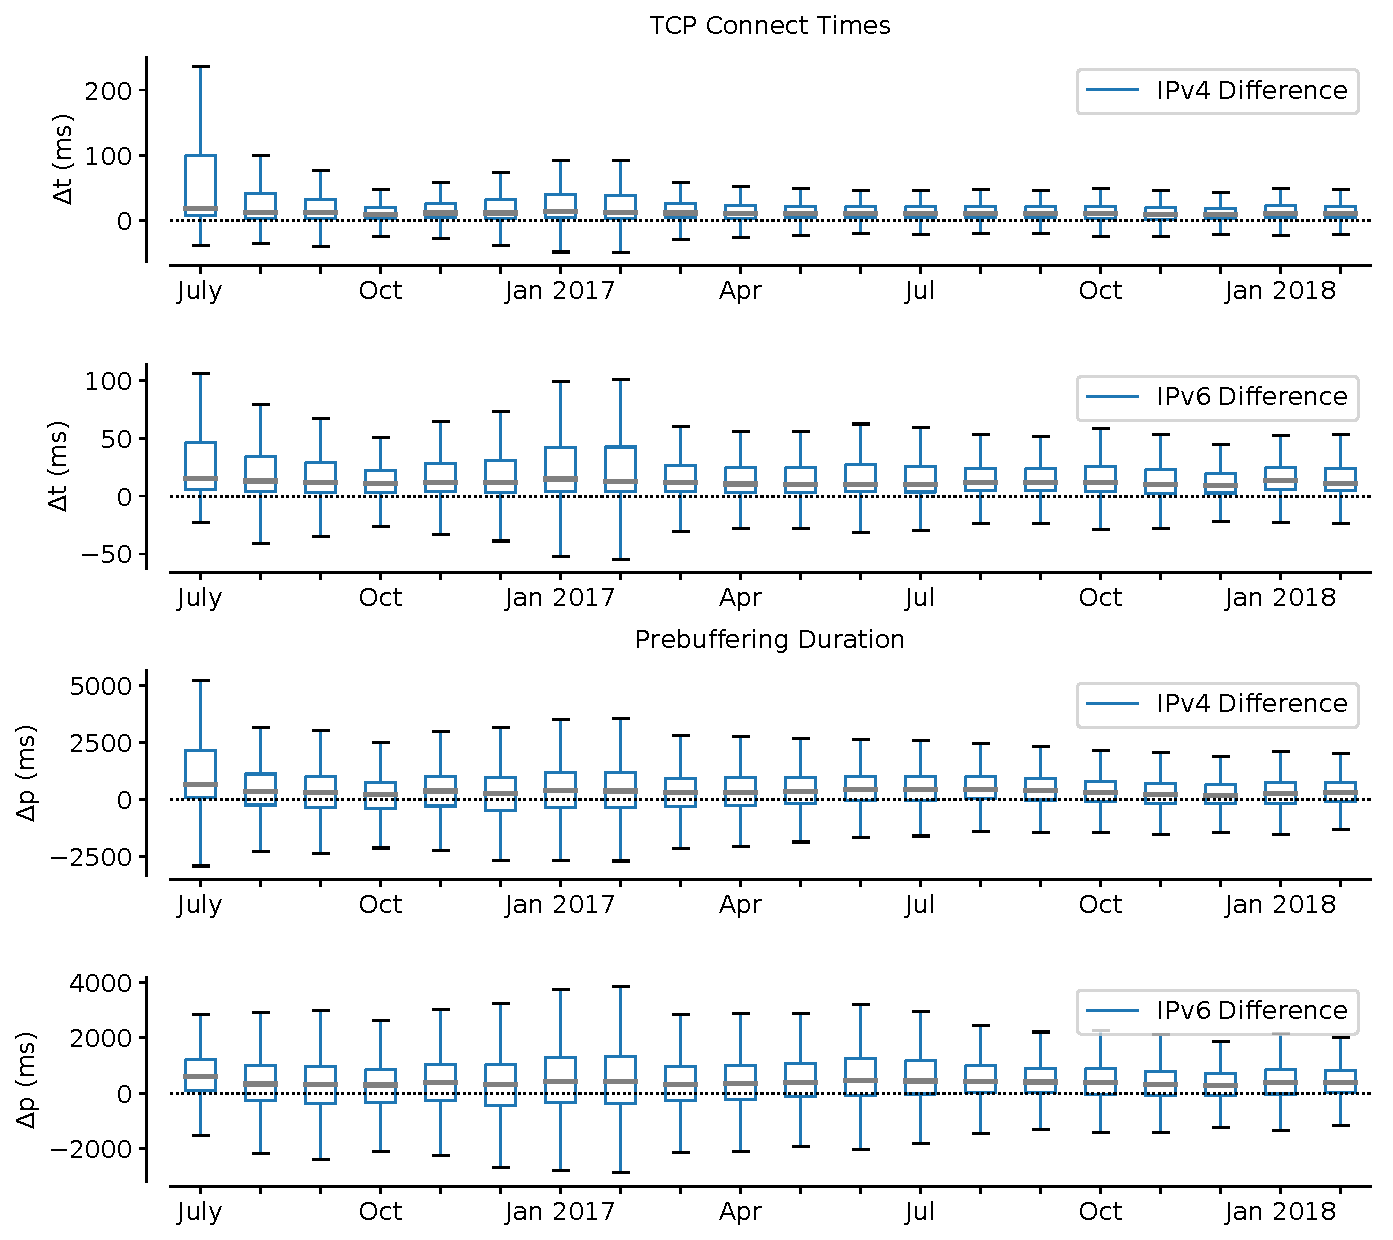
\includegraphics[keepaspectratio, height=8cm, width=15cm]{figures/cache/allisps/netflix-tcp-pd-delay-boxplot-all-isp.pdf}
	\caption[All ISPs TCP Connect Times and Pre-Buffering Duration Boxplot Deltas]{Boxplot of difference for TCP connect times and prebuffering durations over IPv4 and IPv6 between Netflix and ISPs.
	The median line here represents the time series graph in \cref{fig:All ISPs TCP Connect Times and Pre-Buffering Duration Timeseries Deltas}.}
	\label{fig:All ISPs TCP Connect Times and Pre-Buffering Duration Boxplot Deltas}
\end{figure}

To plot the deltas, we followed the same analysis \cite{bajpaimeasuring} did for the Youtueb dataset. To plot the timeseries for these deltas, we calculate the median aggregate on the
TCP connect times and the prebuffering duration across all probes on each day for the difference between Netflix and ISPs.
\cref{fig:All ISPs TCP Connect Times and Pre-Buffering Duration Timeseries Deltas} shows the timeseries of median TCP connect times and prebuffering duration over IPv4 and IPv6 across all probes.
Here, positive values indicate Netflix OCA server requires more connect time and pre-buffering duration as compared to ISPs caches. Latency of around 10-20 ms and higher prebuffering durations (around 0-750 ms or more) are observed for Netflix over both IPv4 and IPv6.
For boxplots in \cref{fig:All ISPs TCP Connect Times and Pre-Buffering Duration Boxplot Deltas}, we have rounded the time to the nearest month. Here, we can see that the median resembles the time series \cref{fig:All ISPs TCP Connect Times and Pre-Buffering Duration Timeseries Deltas}.
To get more vivid analysis, \cref{fig:All ISPs Connect Time and Prebuffering Duration CDF Deltas} shows us the distribution of difference in TCP connect times and prebuffering duration over the whole duration.

For calculating the CDF, we calcualted the deltas and then plotted their CDF. To compare the performance, 
we are measuring the TCP connect times to the Netflix OCA (Open Connect Appliances) server and to the ISPs content caches, 
the distribution here shows that around 84\% of the connections are slower for Netflix OCA servers over IPv4 , and around 85\% of the connections are slower for Netflix over IPv6. 
For prebuffering duration which is the time to fetch 2 seconds of video at the specified bitrate from the content server, here Netflix OCA (Open Connect Appliances) server and ISPs caches,
the distribution shows that 68\% of the connections are slower for Netflix over IPv4, and around 69\% of the connections are slower for Netflix over IPv6.

\begin{figure}
	\centering
	\begin{minipage}{0.5\textwidth}
		\centering
		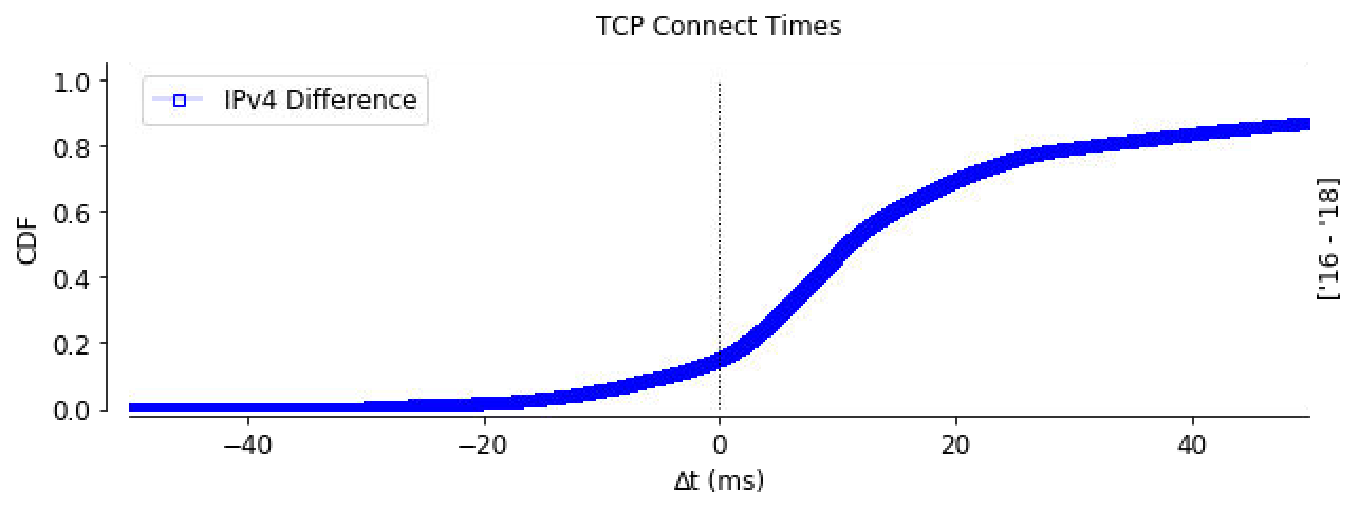
\includegraphics[keepaspectratio, height=5cm, width=8.5cm]{figures/cache/allisps/netflix-syn-diff-all-isps-cdf-v4.pdf}
	\end{minipage}
	\begin{minipage}{0.5\textwidth}
		\centering
		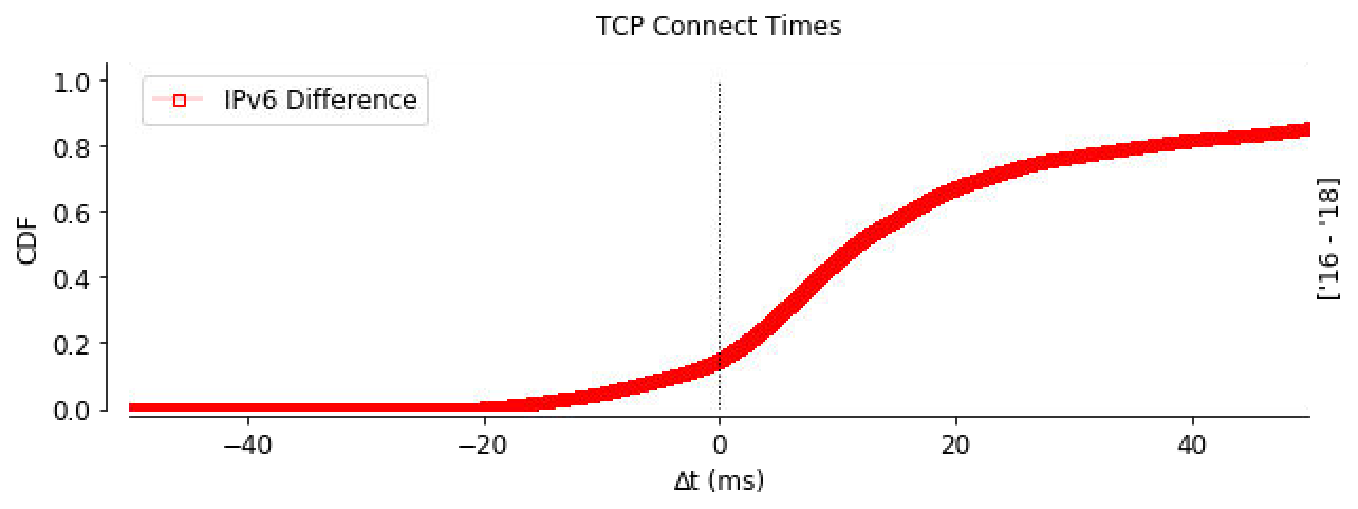
\includegraphics[keepaspectratio, height=5cm, width=8.5cm]{figures/cache/allisps/netflix-syn-diff-all-isps-cdf-v6.pdf}
	\end{minipage}
	\begin{minipage}{0.5\textwidth}
		\centering
		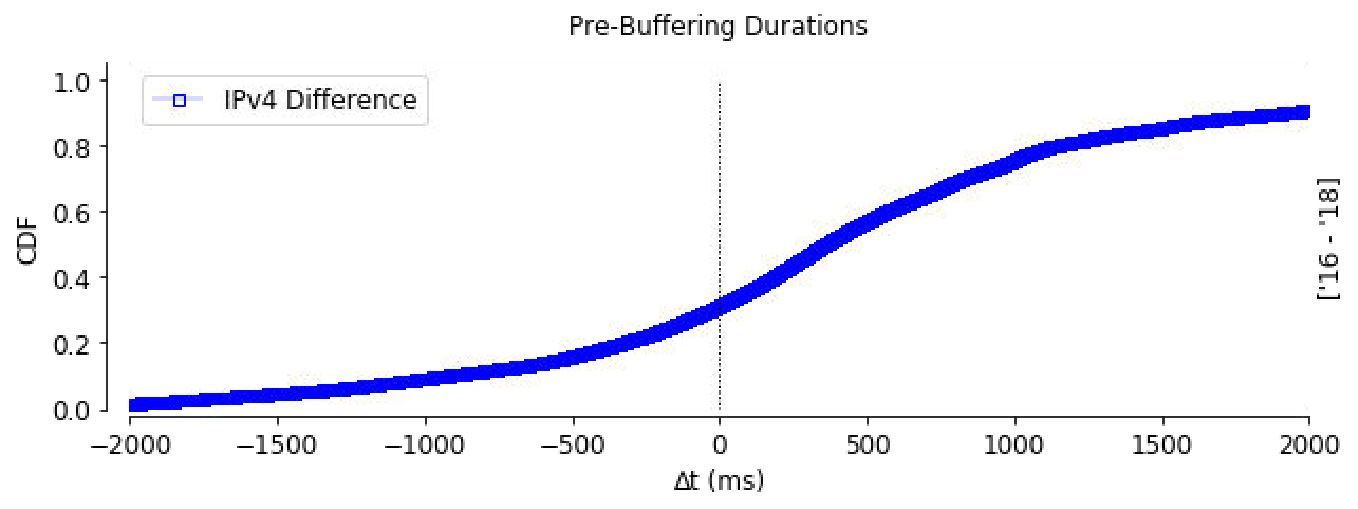
\includegraphics[keepaspectratio, height=5cm, width=8.5cm]{figures/cache/allisps/netflix-pd-diff-all-isps-cdf-v4.pdf}
	\end{minipage}
	\begin{minipage}{0.5\textwidth}
		\centering
		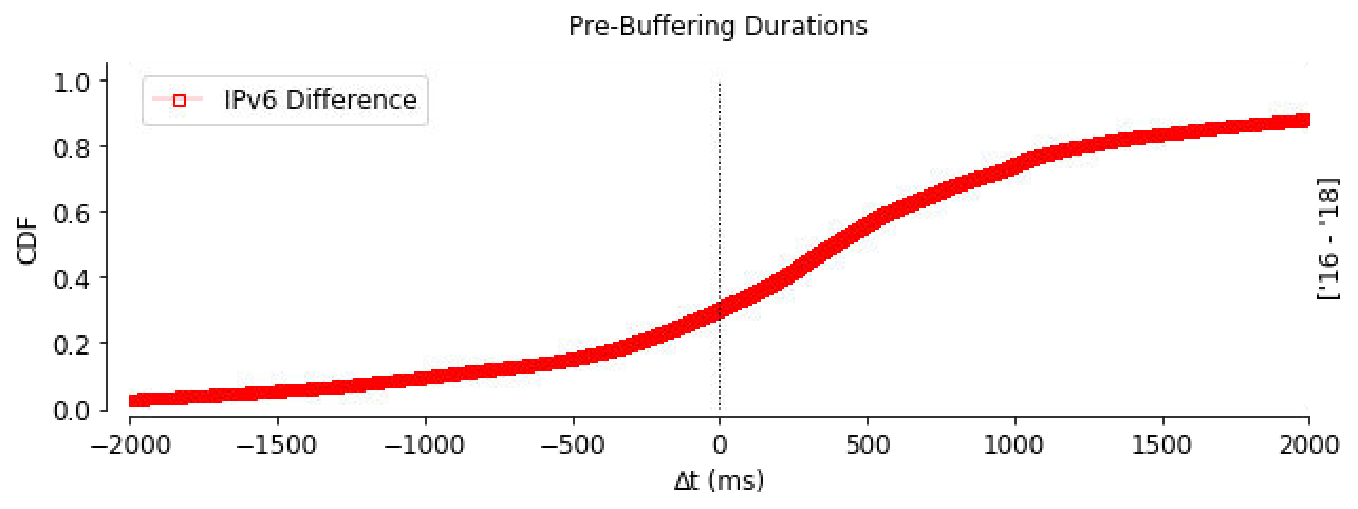
\includegraphics[keepaspectratio, height=5cm, width=8.5cm]{figures/cache/allisps/netflix-pd-diff-all-isps-cdf-v6.pdf}
	\end{minipage}
	\caption[All ISPs Connect Time and Prebuffering Duration CDF Deltas]{CDF of difference of TCP connect times and Prebuffering Durations for Netflix and ISPs over IPv4 and IPv6. The distribution here shows that around 84\% of the connections are slower for Netflix OCA servers over IPv4 , and around 85\% of the connections are slower for Netflix over IPv6. 
For prebuffering duration which is the time to fetch 2 seconds of video at the specified bitrate from the content server, here Netflix OCA (Open Connect Appliances) servers and ISPs caches,
the distribution shows that 68\% of the connections are slower for Netflix over IPv4, and around 69\% of the connections are slower for Netflix over IPv6.}
	\label{fig:All ISPs Connect Time and Prebuffering Duration CDF Deltas}
\end{figure}

\FloatBarrier

\subsection*{Throughput}

\begin{figure}[!ht]
	\centering
	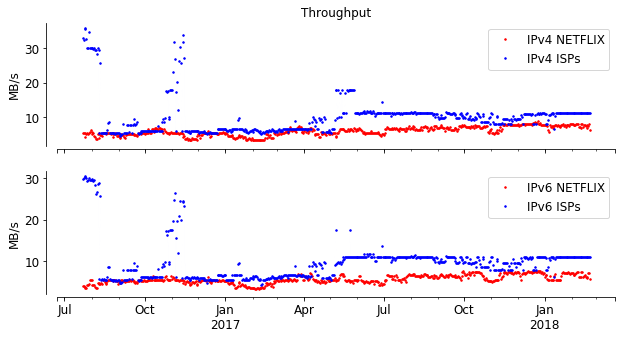
\includegraphics[keepaspectratio, height=5cm, width=15cm]{figures/cache/allisps/netflix-throughput-timeseries-all-isp-separate.png}
	\caption[All ISPs Throughput Timeseries Absolute]{Time series of Throughput for individual address family's i.e. IPv4 and IPv6 for Netflix and ISPs. We are considering 
	the \textit{bytes\_sec} field described in \cref{table:netflix}. As can be seen, the achieved throughput for ISP caches is somwehat comparable or more than Netflix OCA server.}
	\label{fig:All ISPs Throughput Timeseries Absolute}
\end{figure}

\begin{figure}[!ht]
	\centering
	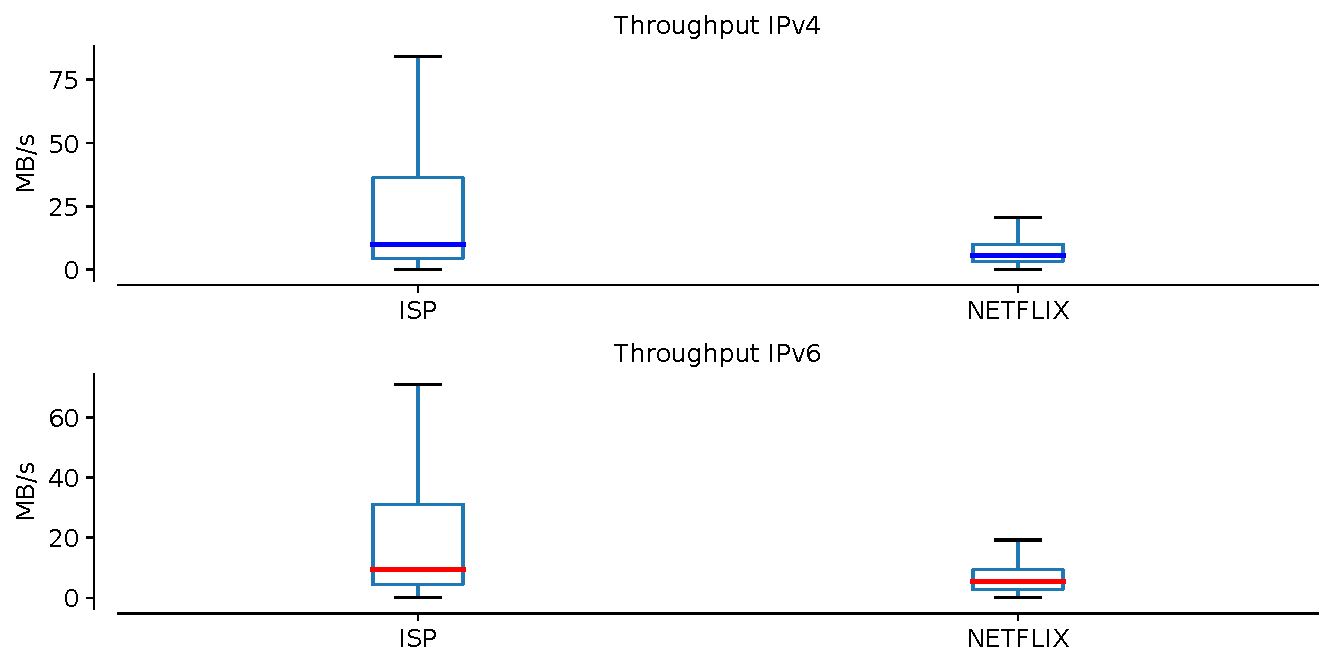
\includegraphics[keepaspectratio, height=5cm, width=15cm]{figures/cache/allisps/netflix-throughput-boxplot-all-isp-separate.pdf}
	\caption[All ISPs Throughput Boxplot Absolute]{Boxplot of Throughput for individual address family's i.e. IPv4 and Ipv6 for Netflix and ISPs. The median line here shows that the achieved throguhput is
	comparable but the thrid quartile of ISP caches shows that the achieved throughput is higher for ISPs over both address family's.}
	\label{fig:All ISPs Throughput Boxplot Absolute}
\end{figure}

After comparing the TCP connect times and Pre-Buffering duration for Netflix and ISPs, we now know that clients take higher TCP connect times and prebuffering duration
for Netflix OCA servers as compared to the ISPs caches over both the address family's. We will now be comparing the achieved throughput over IPv4 and IPv6 for Netflix OCA server and ISP caches.
We will first look into the individual performance of IPv4 and IPv6 for Netflix and ISPs and then will look into their deltas. \cref{fig:All ISPs Throughput Timeseries Absolute} gives the time series for
both the address families for ISPs and Netflix, and as can be seen, the achieved throughput for ISPs caches is somwehat comparable or more than Netflix OCA server.
We are considering the \textit{bytes\_sec} field from the Netflix \cref{table:netflix}, and we are taking the median aggregate across
all probes on each day. Also, the throughput for IPv4 and IPv6 lies between 0-40 MB/s for ISP caches. To get more deeper insights
we also did the boxplot for IPv4 and IPv6 throughput for ISPs and Netflix, and as can be seen in \cref{fig:All ISPs Throughput Boxplot Absolute} the monthly
throughput variation over IPv4 and IPv6. The median line here shows that the achieved throguhput is comparable but the third quartile of ISPs shows that the achieved throughput is higher for ISP caches over both address family's. We have 
converted the \textit{bytes\_sec} field into MB/s to get a more realistic view. \cref{fig:SKY UK Throughput CDF Absolute} shows the CDF of
throughput over IPv4 and IPv6. We followed the same steps here, and plotted the CDF of \textit{bytes\_sec} field. The CDF here shows that around 80\% of the probes achieved a throughput of 40 MB/s for ISPs over IPv4, whereas for Netflix this is only 10 MB/s
for similar number of probes. For IPv6, 80\% of the probes achieved the throughput of 40 MB/s, while for Netflix this was only 10 MB/s for similar number of probes. 
We will now look into the deltas to get better comparison between ISP caches and Netflix OCA servers.

\begin{figure}[!ht]
	\centering
	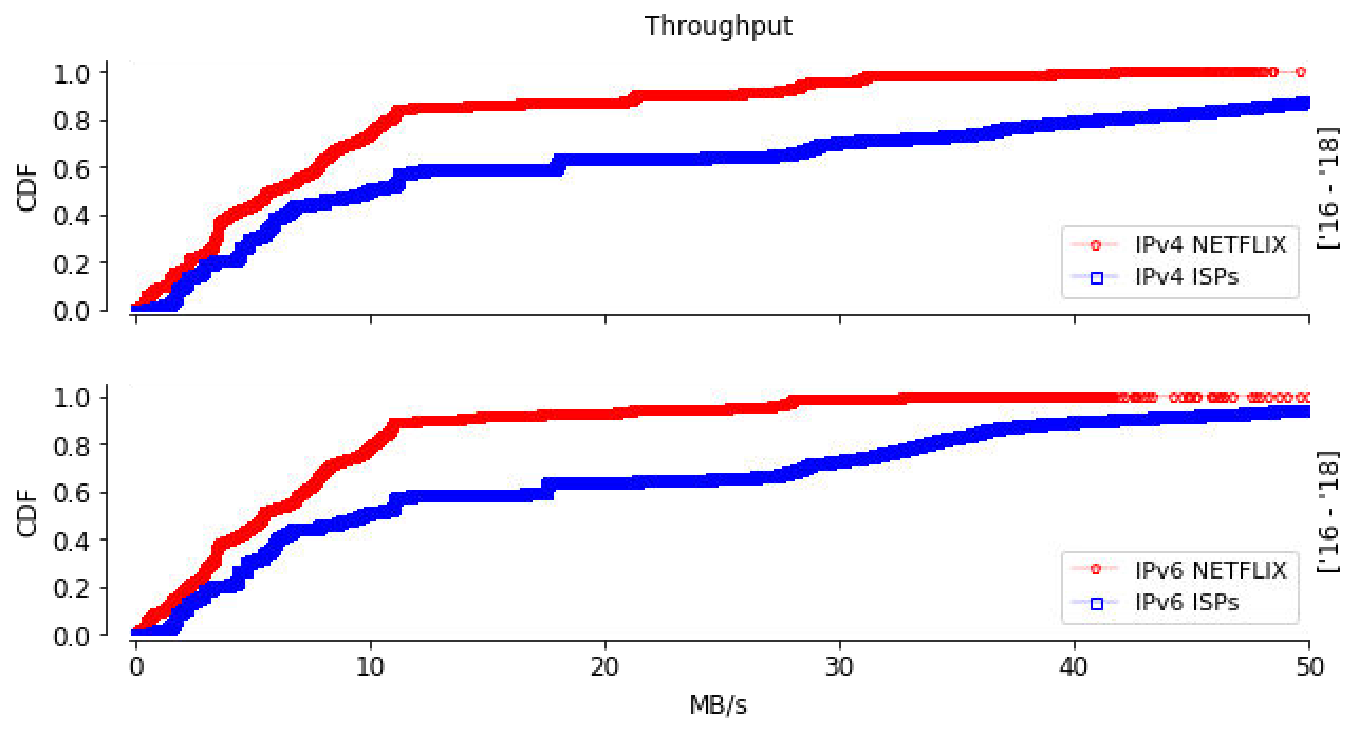
\includegraphics[keepaspectratio, height=5cm, width=15cm]{figures/cache/allisps/netlflix-throughput-difference-all-isps-separate.pdf}
	\caption[All ISPs Throughput CDF Absolute]{CDF of Throughput over IPv4 and IPv6. We followed the same steps here, and plotted the CDF of \textit{bytes\_sec} field. The CDF here shows that around 80\% of the probes achieved a throughput of 40 MB/s for ISPs over IPv4, whereas for Netflix this is only 10 MB/s
for similar number of probes. For IPv6, 80\% of the probes achieved the throughput of 40 MB/s, while for Netflix this was only 10 MB/s for similar number of probes.}
	\label{fig:All ISPs Throughput CDF Absolute}
\end{figure}

\FloatBarrier

\begin{figure}[!ht]
	\centering
	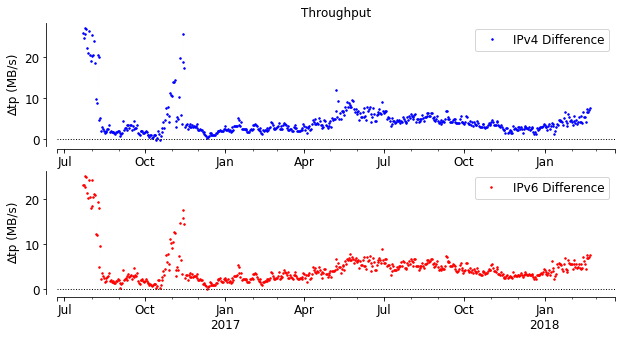
\includegraphics[keepaspectratio, height=5cm, width=15cm]{figures/cache/allisps/netflix-throughput-timeseries-all-isps.png}
	\caption[All ISPs Throughput Timeseries Deltas]{Time series of median aggregate of throughput across all probes over each day.
We can see that the difference is positive, indicating a higher throughput for ISP caches, also the difference lies between 0-30 MB/s.}
	\label{fig:All ISPs Throughput Timeseries Deltas}
\end{figure}

\begin{figure}[!ht]
	\centering
	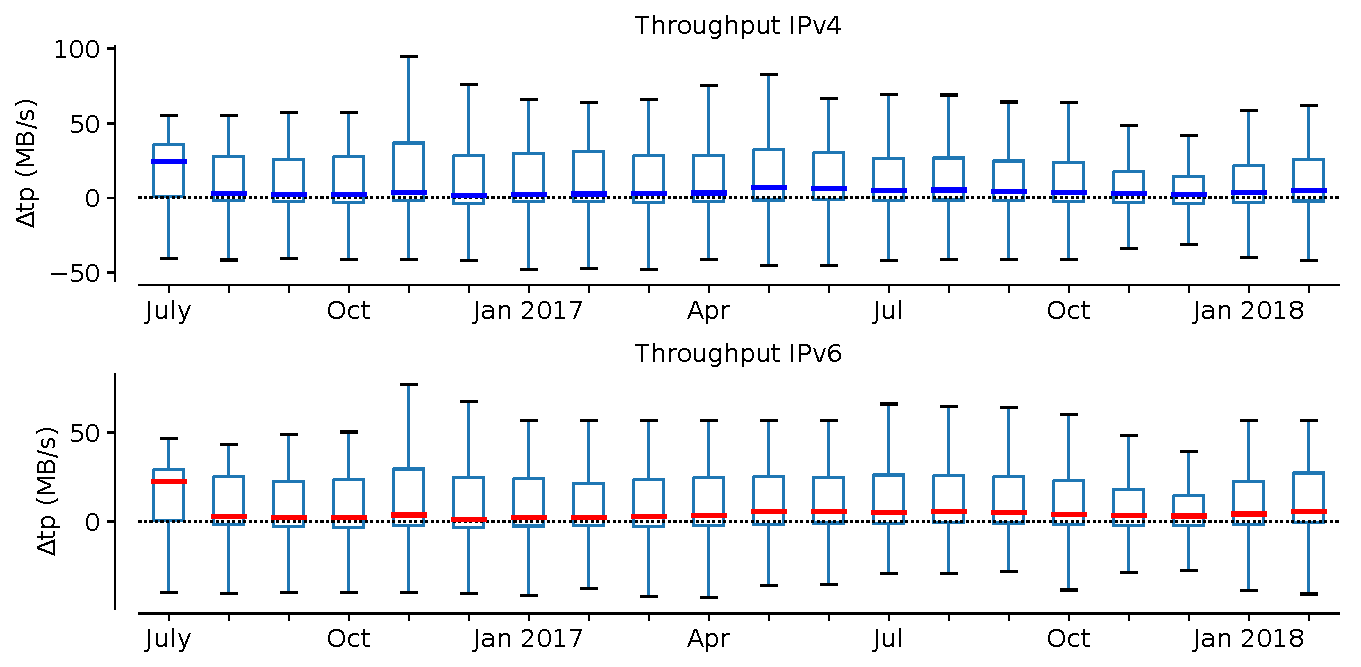
\includegraphics[keepaspectratio, height=5cm, width=15cm]{figures/cache/allisps/netflix-throughput-boxplot-all-isps.pdf}
	\caption[All ISPs Throughput Boxplot Deltas]{Boxplot of difference of throughput over IPv4 and IPv6 between ISP caches and Netflix OCA server. The median line shows similar curves as the time series \cref{fig:All ISPs Throughput Timeseries Deltas}, depicting higher throughput for ISPs over both address families.}
	\label{fig:All ISPs Throughput Boxplot Deltas}
\end{figure}

\subsection*{Deltas}

Before starting with the deltas, we would live to define the terminologies we used to get the results. We are considering the \textit{bytes\_sec} field only and using the same terminilogy Bajpai et al. used in \cite{bajpaimeasuring}. We denote the throughput 
over IPv4 for ISPs as \textit{tp(y}) and throughput over IPv4 for Netflix as \textit{tp(x)}, then the \textit{delta} will be $\Delta$tp = tp(y) - tp(x).
To plot the deltas, we first start with the time series, and \cref{fig:All ISPs Throughput Timeseries Deltas} shows us the time series of median aggregate of throughput across all probes over each day.
We can see that the difference is positive, indicating a higher throughput for ISP caches, also the difference lies between 0-30 MB/s.
\cref{fig:All ISPs Throughput Boxplot Deltas} shows the boxplot of difference of throughput over IPv4 and IPv6 between ISP caches and Netflix OCA server. The median line shows similar curves as the time series \cref{fig:All ISPs Throughput Timeseries Deltas}, depicting higher throughput for ISPs over both address families.
To get a more clear picture about the performance, we plot the CDF of \textit{bytes\_sec} field. 
\cref{fig:All ISPs Throughput CDF Deltas} shows the CDF of difference of throughput over IPv4 and IPv6 for ISPs and Netflix. 
Around 66\% of the times, ISP caches achieved higher throughput than Netflix over IPv4 and IPv6.

\begin{figure}[!ht]
	\centering
	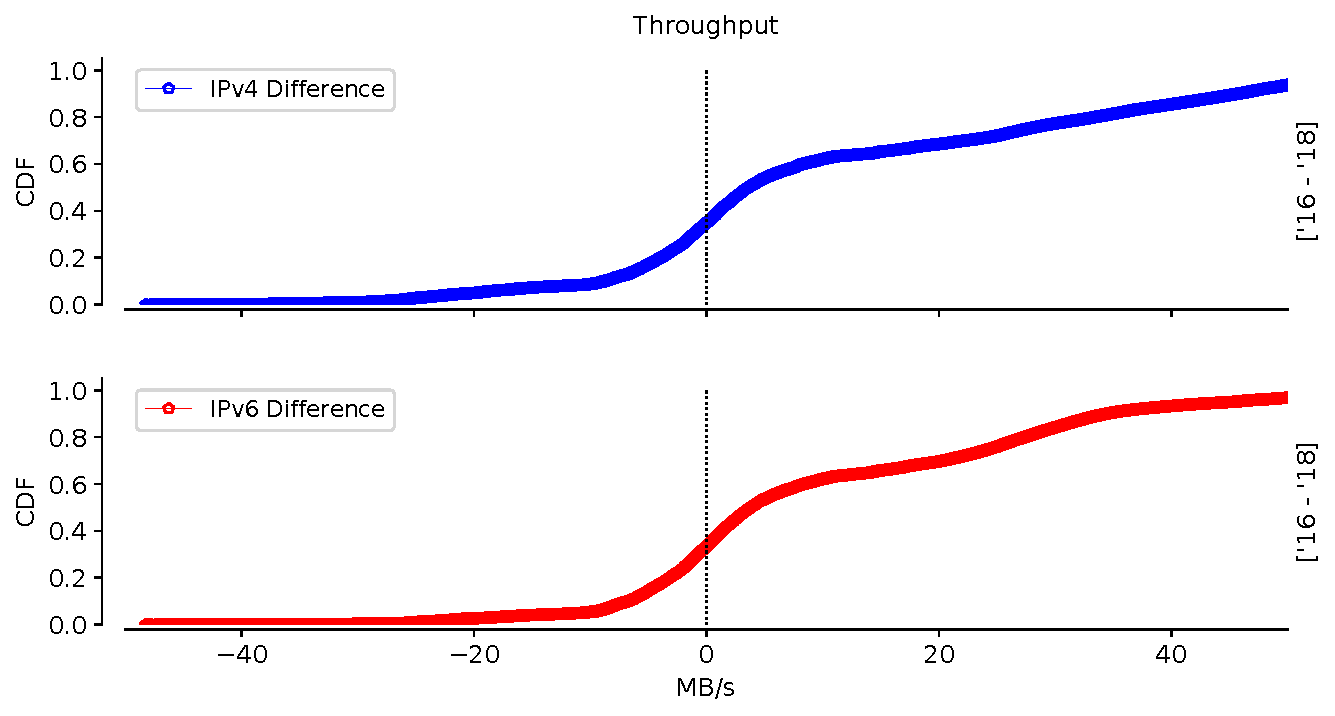
\includegraphics[keepaspectratio, height=5cm, width=15cm]{figures/cache/allisps/netlflix-throughput-difference-all-isps.pdf}
	\caption[All ISPs Throughput CDF Deltas]{CDF of difference of throughput over IPv4 and IPv6 for ISPs and Netflix. 
Around 66\% of the times, ISP caches achieved higher throughput than Netflix over IPv4 and IPv6.}
	\label{fig:All ISPs Throughput CDF Deltas}
\end{figure}

\FloatBarrier